\documentclass[accentcolor=tud0b,12pt,paper=a4]{tudreport}

\usepackage[utf8]{inputenc}
\usepackage{ngerman}
\usepackage{parcolumns}
\usepackage{color}
\usepackage{listings}
\usepackage[section]{placeins}
\usepackage{pdfpages}

\definecolor{javablue}{rgb}{0,0,0.4} % for strings
\definecolor{javapurple}{rgb}{0.5,0,0.35} % keywords
\definecolor{javagreen}{rgb}{0,0.35,0} % comments

\lstset{
  language=Java,
  breaklines=true,
  breakatwhitespace=true,
  frame=single,
  stringstyle=\ttfamily,
  numbers=left,
  numberstyle=\tiny,
  showstringspaces=false,
  basicstyle=\footnotesize,
  keywordstyle=\color{javapurple},
  stringstyle=\color{javablue},
  commentstyle=\color{javagreen}
}

\usepackage{hyperref}
\hypersetup{
    colorlinks=true,
    linkcolor={black},
    urlcolor={blue}
}

\newcommand{\titlerow}[2]{
	\begin{parcolumns}[colwidths={1=.15\linewidth}]{2}
		\colchunk[1]{#1:} 
		\colchunk[2]{#2}
	\end{parcolumns}
	\vspace{0.2cm}
}

% keine Worttrennung mit Bindestrich für die folgenden Worte
\hyphenation{Nightscout}
\hyphenation{Coverity}
\hyphenation{Pull-Request}
\hyphenation{GitHub}
\hyphenation{Interface}

\title{Open Diabetes UAM Heuristik Algorithmen}
\subtitle{Qualitätssicherungsdokument}
\subsubtitle{%
	\titlerow{Gruppe 11}{%
		Aino Schwarte <aino.schwarte@stud.tu-darmstadt.de>\\
		Anna Mees <anna.mees@stud.tu-darmstadt.de>\\
		Jan Paul Petto <janpaul.petto@stud.tu-darmstadt.de>\\
		Paul Wolfart <paul.wolfart@stud.tu-darmstadt.de>\\
		Tom Großmann <tom.grossmann@stud.tu-darmstadt.de>}
	\titlerow{Teamleiter}{Benedikt Schneider <schneider-benedikt@gmx.net>}
	\titlerow{Auftraggeber}{%
		M.Sc. Jens Heuschkel <heuschkel@tk.tu-darmstadt.de>\\
		Telecooperation\\
		Smart Urban Networks}
	\titlerow{Abgabedatum}{31.03.2019}
\institution{Bachelor-Praktikum WS 2018/2019\\Fachbereich Informatik}}

\begin{document}

	\maketitle
	\tableofcontents 
	
	\chapter{Einleitung}
	%	\textcolor{gray}{Kurze Projektbeschreibung}\\
Das sogenannte Un-Announced-Meal-Problem (UAM) ist derzeit eine der größten Therapieschwächen bei der Behandlung von Diabetes Mellitus \mbox{Typ 1}\footnote{Diabetes Typ 2 fällt nicht unter das UAM-Problem, da es sich dabei lediglich um eine Insulinresistenz handelt. Eine nicht erkannte Mahlzeit stellt also ein geringeres Risiko dar und die Krankheitsbilder lassen sich auch nicht direkt vergleichen.} und beschreibt die Mahlzeiten, welche vom Patienten nicht berücksichtigt wurden und somit den Blutzuckerspiegel unkontrolliert steigen lassen. Denn bei Diabetespatienten produziert der Körper kaum bis gar kein eigenes Insulin, welches den Blutzuckerpegel reguliert. Das Insulin muss manuell verabreicht werden. Neben der Grundversorgung wird zusätzlich auch eine zu jeder Mahlzeit präzise berechnete Insulindosis benötigt,  um den Blutzuckerspiegel innerhalb akzeptabler Grenzwerte zu halten. Extrem hohe oder niedrige Blutzuckerwerte können akute schwerwiegende und sogar tödliche Folgen haben. Befindet sich der Blutzuckerspiegel regelmäßig und über längere Zeiträume außerhalb der Normalwerten, kann dies auch zu schweren Langzeitschäden führen.

Um in Zukunft ein voll automatisches System mit Messgerät und Insulinpumpe zu ermöglichen, welches die Insulinversorgung des Patienten übernimmt, wird eine Möglichkeit benötigt, Mahlzeiten verlässlich zu erkennen. Bisherige Systeme können mit der Problematik von unangekündigten Mahlzeiten nicht umgehen, wenn eine Mahlzeit vom Patienten vergessen oder zu gering eingeschätzt wurde. Das dadurch fehlende Insulin wird bestenfalls allmählich mit dem steigendem Blutzuckerspiegel verabreicht, was allerdings zu spät ist, um hohe Werte zu verhindern. In solchen Situationen kann es zu einer lebensbedrohlichen Überkorrektur kommen.

Das Ziel unseres Projekts ist es anhand des steigenden Blutzuckers mit wenigen Messwerten eine Mahlzeit präzise zu berechnen, damit die adäquate Menge an Insulin schon frühzeitig injiziert werden kann. Dazu bauen wir auf dem Open Source Projekt Nightscout\footnote{\url{http://www.nightscout.info}} auf, welches der Visualisierung von gemessenen Blutzuckerwerten dient. Die Messungen werden alle fünf Minuten von einem Sensor unter der Haut durchgeführt. Über die Cloud werden sie in einer Datenbank gespeichert und können auf jedem internetfähigen Gerät abgerufen werden. Zusätzlich werden Insulindosierungen und bekannte Mahlzeiten als Events kenntlich gemacht. Unser Programm bezieht diese Messwerte und Events aus der Datenbank und startet einen Algorithmus zur Berechnung von Mahlzeiten. Da es keine bekannte optimale Methode gibt, um Mahlzeiten zu erkennen, implementieren wir unterschiedliche Ansätze, aus denen gewählt werden kann. Diese Ansätze beruhen auf verschiedenen wissenschaftlichen Publikationen, welche die Auswirkungen von Kohlenhydraten und Insulin auf den Blutzuckerspiegel mathematisch beschreiben. Wir benutzen diese Modelle um von den gemessenen Blutzuckerwerten und bekannten Insulinbehandlungen auf Kohlenhydraten, also Mahlzeiten, zurück zu schließen. Die berechneten Mahlzeiten werden dann als neue Events in Nightscout eingetragen und je nach Ansatz auch im weiteren Verlauf berücksichtigt.

Es ist nicht sicher, ob sich das UAM-Problem mit dem aktuellen Sachverstand der Wissenschaft zuverlässig lösen lässt. Unsere Ansätze können höchstens so gut sein, wie die Modelle, die uns zur Verfügung stehen. Unser Projekt dient also als Plausibilitätsprüfung, ob sich das UAM-Problem zurzeit realistisch lösen lässt. Wir werden unsere Algorithmen, wenn sie sich als verlässlich erweisen, der Nightscout Community zur Verfügung stellen.


	\chapter{Qualitätsziele}
    \section{Korrektheit}
    
	\subsection{Beschreibung}
Unser wichtigstes QS-Ziel ist die Korrektheit. Dabei liegt das Hauptaugenmerk neben der Erzeugung von korrekten Daten auch darauf, Fehler und Fehlerquellen korrekt zu erkennen. Wenn die zur Verfügung stehenden Daten zur Berechnung einer Mahlzeit nicht ausreichen oder sonstige Probleme auftreten, muss der Benutzer darüber in Kenntnis gesetzt werden und es dürfen keine potentiell falschen Ergebnisse produziert werden. Diabetespatienten, die unsere Algorithmen verwenden werden, vertrauen darauf, dass unser Ansatz korrekte Werte zurück gibt und Mahlzeiten richtig erkannt werden. Da ein zu hoher oder zu niedriger Insulinwert, wie bereits erläutert, schwere körperliche Langzeitfolgen haben oder sogar akut lebensbedrohlich sein kann, ist es offensichtlich, weshalb hier keine Fehler passieren dürfen.

	\subsection{Maßnahmen}
Wir wollen die Korrektheit durch die die Nutzung von automatischen Coverity Scans\footnote{\url{https://scan.coverity.com}} und dem Continuous Integration Tool Travis CI\footnote{\url{https://travis-ci.org}} erreichen. Travis CI kann kostenlos genutzt werden, da wir an einem Open-Source-Projekt arbeiten, welches auf GitHub\footnote{\url{http://github.com/TUDa-BP-11/opendiabetes-uam-heuristik}} veröffentlicht wird.

Travis CI kompiliert die Software und überprüft automatisch alle implementierten Tests und meldet zurück, ob diese erfolgreich abgeschlossen wurden. 

Coverity Scans analysieren den Code auf Race Conditions und Speicherlecks, bei denen zwar Arbeitsspeicher belegt, allerdings weder genutzt, noch frei gegeben wird. 

Wir verwenden mehrere Branches für zu entwickelnde Features und einen Master Branch, auf dem immer eine lauffähige Version liegt. Auf dem Master Branch kann nicht direkt gepusht werden, nur über die Feature Branches. Es sind Pull-Request-Reviews und Status Checks nötig, um auf den Master Branch zu schreiben. Diese Status Checks beinhalten das erfolgreiche Kompilieren des Codes durch Travis CI und den erfolgreichen Durchlauf aller Tests. Erst im Anschluss können Pull-Requests akzeptiert werden. Wenn mindestens eine andere Person den Pull-Request überprüft und akzeptiert hat, wird der Branch gemerged. Git führt einen Verlauf, wer den Pull-Request-Review freigegeben hat. Es wird somit immer protokolliert, wer Korrektur gelesen hat. Dieses Protokoll wird im Anhang zur Verfügung gestellt.


	\subsection{Prozessbeschreibung}
In GitHub gibt es einen Master Branch. Entwickelt wird ausschließlich in sogenannten Feature Branches. Für jedes Feature bzw. jede Feature-Gruppe wird ein eigener Branch erstellt. Nach Abschluss des Features und der Iterationszyklen wird ein Pull-Request erstellt. Mindestens eine andere Person im Projekt kontrolliert die Änderungen im Pull-Request, bevor dieser akzeptiert wird. Werden Mängel oder Probleme entdeckt, löst diese die Person, die den Pull-Request erstellt hat. Dies soll innerhalb der nächsten drei Tage geschehen und darf maximal auf sieben Tage verlängert werden. Sollte nach dieser Zeit noch keine Lösung gefunden werden, wir dies beim nächsten Auftraggebertreffen besprochen. Treten dabei Probleme oder Schwierigkeiten auf, wird die Hilfe der Teammitglieder in Anspruch genommen. Danach werden die Änderungen erneut von mindestens einer anderen Person kontrolliert, bis keine Mängel mehr gefunden werden und der Branch in den Master Branch gemerged werden kann. 

Travis CI wird automatisch bei jedem Git-Commit ausgeführt. Dafür wurde eine entsprechende .travis.yml Datei angelegt. Travis CI kompiliert die Software und startet alle implementierten Tests. Schlägt einer der Tests fehl, werden wir per E-Mail informiert. Außerdem vergibt \mbox{Travis CI} Badges, anhand derer in GitHub sichtbar ist, welche Branches in ihrem aktuellen Stand ohne Probleme kompiliert und getestet wurden.

Die Tests bestehen aus statischen Unit-Tests, welche zunächst alle grundlegenden Funktionen testen, ohne welche die anderen Funktionen nicht arbeiten können, wie zum Beispiel das korrekte Verbinden auf eine Nightscout Test Instanz und die volle Funktionalität der API-Schnittstelle. Außerdem werden alle verwendeten mathematischen Modelle - zum Beispiel zur Berechnung von Insulinabbau über Zeit im Blutkreislauf - mit festen Testdaten auf Korrektheit überprüft. Diese Testdaten wurden zuvor unabhängig von der Implementierung der Funktionen berechnet, wir testen die Funktionen also nicht mit Werten, die durch die Funktionen selbst generiert wurden. In einem zweiten Schritt werden - abhängig vom Status und Inhalt der in der Nightscout Test Instanz gespeicherten Daten - dynamisch weitere Tests generiert, die die implementierten Algorithmen auf verschiedene Weisen testen. Dies ist stark von den jeweiligen Algorithmen abhängig, wir testen aber mindestens jede offen verfügbare (\texttt{public}) Methode. Dafür verwenden wir die in JUnit-5 integrierte dynamische Test-Generation. Methoden die nicht automatisch getestet werden können müssen durch Tests des Erstellers getestet werden. Dies stellt sicher, dass sie fehlerfrei funktionieren. Sollten hierbei Fehler auftreten, werden diese mit sinnvollen Fehlermeldungen ausgegeben, so dass diese behoben werden können und der Nutzer informiert ist. Auf diese Weise können wir Tests mit verschiedenen Beispieldaten problemlos mehrmals ausführen und auch die Möglichkeit anbieten, das Programm mit eigenen Testdaten zu überprüfen. 

Sollte die Test Instanz von Nightscout einmal nicht verfügbar sein, schlagen die Tests mit eindeutigen Meldungen fehl und teilen dem Benutzer mit, wie die Fehler zu beheben sind. Wenn auf der Nightscout Test Instanz unzureichende oder falsche Daten gespeichert sind, überprüfen die Tests, ob die Algorithmen korrekt abbrechen und dem Benutzer mitteilen, welche Probleme mit den verfügbaren Daten bestehen. Nicht ausgeführte Tests auf Grund von fehlenden Daten in der Nightscout Test Instanz  werden als nicht ausgeführt markiert, lassen den gesamten Test aber nicht fehlschlagen.

Coverity wird nur bei Commits auf den Coverity Branch ausgeführt, da die Nutzung von Coverity beschränkt ist. Dies wird durchgeführt, bevor in den Master Branch gemerged wird. Die Anzahl der Builds pro Woche ist auf 28 mit maximal 4 Tests am Tag beschränkt, wenn weniger als 100.000 Zeilen Code getestet werden. Wurden die maximale Anzahl der Builds pro Tag erreicht, werden weitere Builds an dem entsprechenden Tag abgelehnt. Wenn Travis CI oder Coverity Fehler erzeugen, müssen diese von demjenigen, der gepusht hat. Auch dies soll innerhalb der nächsten drei Tage geschehen und kann ebenfalls maximal auf sieben Tage verlängert werden. Falls dies nicht gelöst werden kann wird das Problem auf dem nächsten Aufraggebertreffen besprochen.

\newpage

\section{Modularität}

\subsection{Beschreibung}

Unser zweites QS-Ziel ist die Modularität und damit verbunden die Erweiterbarkeit. Unser Ziel ist es, ohne viel Aufwand neue Algorithmen zur Berechnung der Mahlzeiten einpflegen zu können, sowie die Möglichkeit zu bieten neue Daten und Datenquellen einbinden zu können.

Dies ist besonders sinnvoll, da unser Code einer Opensource-Community, unter der \mbox{AGPLv3} Lizenz, auf GitHub zur Verfügung steht und Mitglieder der Nightscout-Community (einschließlich Herrn Heuschkel als Auftraggeber) den Code wieder verwenden möchten.

So ist es möglich, wenn neue Ansätze für eine bessere Berechnung von Mahlzeiten gefunden wurden, diese einfach zu implementieren und auszuführen, ohne dass das Hauptprogramm geändert werden muss. Genauso können neue Datenquellen, wie zum Beispiel eine MySQL Datenbank, oder ein entferntes Dateisystem, eingefügt werden.

\subsection{Maßnahmen}

Um dies möglich zu machen, werden zunächst GitHub Wiki Artikel zur Verfügung gestellt\footnote{\url{https://github.com/TUDa-BP-11/opendiabetes-uam-heuristik/wiki}}. In diesen wird ausführlich erklärt, wie unsere Software zu installieren, verwenden und erweitern ist. Die Projektstruktur ist modular, sodass neue Algorithmen und Datenquellen einfach durch die Implementierung eines Interfaces hinzugefügt werden können. Es werden verschiedene Entwurfsmuster (Design Patterns) verwendet, um die Erweiterbarkeit sicher zu stellen.

Unser Projekt gliedert sich in drei Hauptmodule: Das Hauptprogramm \mbox{(Modul 1)}, die Anbindung an Nightscout und der Daten-Parser \mbox{(Modul 2)} und die Repräsentation der Daten \mbox{(Modul 3)}. Diese Module können unabhängig voneinander verwendet werden, wobei sie jeweils auf das in der obigen Liste folgende Modul aufbauen. Unser Auftraggeber verwendet zum Beispiel die im dritten Modul definierten Datenklassen auch für andere Projekte, und die Anbindung an Nightscout kann benutzt werden, um beliebige Daten von und zu Nightscout zu übertragen.

Das Hauptprogramm gliedert sich in vier weitere Module: Die Hauptklasse und ihre dazugehörigen Klassen, zum Starten des Programms \mbox{(Modul 1.1)}, die Datenquellen, zum Einlesen und Abspeichern der Daten \mbox{(Modul 1.2)} und die Algorithmen, zur Verarbeitung der Daten \mbox{(Modul 1.3)}. Häufig benutzte Funktionen und die Implementierungen der verwendeten mathematischen Modelle, welche in verschiedenen Algorithmen benötigt werden, werden in eigene Klassen ausgelagert \mbox{(Modul 1.4)}. Hierunter fällt zum Beispiel das Berechnen von Insulinabbau im Blutkreislauf über Zeit oder die Umwandlung von Kohlenhydraten zu Glucose über Zeit, was unabhängig vom später verwendeten Algorithmus immer gleich verläuft. Dies ermöglicht es viele Funktionen in verschiedenen Algorithmen wieder zu verwenden und diese unabhängig von den Algorithmen testen zu können.

Wie bereits beim Ziel der Korrektheit beschrieben, werden Pull-Requests auf den Master Branch von mindestens einer anderen Person kontrolliert. Hier wird auch überprüft, ob die oben beschriebene Modularität eingehalten wurde.

\subsection{Prozessbeschreibung}

Die Wiki Artikel beschreiben auf englisch, Schritt für Schritt, wie ein neuer Algorithmus implementiert werden kann. Dies wird exemplarisch an einem unserer Algorithmen gezeigt. Die Artikel werden von zwei Projektmitgliedern geschrieben. Mindestens zwei andere Mitglieder lesen diese Korrektur und überprüfen anhand einer Checkliste (siehe Anhang), ob diese vollständig sind und vollziehen die Schritte auf einem neuen System nach. Dies ist erreicht, wenn der Algorithmus nach der Ausführung der Anleitung lauffähig ist.

Sowohl für die Algorithmen als auch für die Datenquellen verwenden wir das \mbox{Strategy Pattern}\footnote{\url{https://en.wikipedia.org/wiki/Strategy_pattern}}, um während der Laufzeit verschiedene Algorithmen und Datenquellen zu laden. Das Datenquellen-Interface \mbox{(\texttt{DataProvider})} definiert abstrakte Methoden zum Laden von Blutzucker Messwerten, Insulinbehandlungen, und bekannten Mahlzeiten jeweils in einem bestimmten Zeitfenster. Das Algorithmus-Interface \mbox{(\texttt{Algorithm})} definiert abstrakte Methoden, um bekannte Blutzucker Messwerte, Insulinbehandlungen und Mahlzeiten zur Verfügung zu stellen, eine Methode um die Ausführung des Algorithmus zu starten und eine Methode um die berechneten Mahlzeiten abzurufen.

Die Nightscout Anbindung beinhaltet einen unabhängig verwendbaren Parser, welcher ebenfalls ein Interface erweitert und mit dem Template Method Pattern das direkte Analysieren von Strings (zum Beispiel die Rückgabewerte der Nightscout API) und die Verwendung von normalen Textdateien als Quelle ermöglicht. Dieser Parser kann die JSON-Repräsentation der Daten von Nightscout übersetzen. Da Nightscout selbst das Hinzufügen von neuen Datentypen erlaubt, ist es auch hier kein Problem einen neuen Parser für noch unbekannte Daten hinzuzufügen.

Zur Repräsentation der Daten im Programm benutzen wir verschiedene vom Auftraggeber vorgegebene Datenklassen, welche auch in anderen Projekten des Auftraggebers verwendet werden. Alle Algorithmen und Datenquellen benutzen ausschließlich diese Klassen, um miteinander zu kommunizieren, und ermöglichen dadurch ebenso unser Programm mit anderen vom Auftraggeber verwendeten Programmen zu kombinieren.

Bei der Kontrolle von Pull-Requests auf den Master Branch achtet die kontrollierende Person\footnote{Die kontrollierende Person ist immer eine andere, als die Person, welche einen Pull-Request erstellt hat. Dies wird von GitHub sicher gestellt, der Ersteller eines Pull-Requests ist automatisch nicht mehr in der Lage, den Pull-Request anzunehmen.} darauf, dass die verwendeten Entwurfsmuster korrekt umgesetzt wurden und zum Beispiel ein Algorithmus nicht direkt Daten an das Hauptprogramm weiter gibt. Außerdem wird darauf geachtet neue Funktionen so abstrakt wie möglich zu implementieren, um die Wiederverwendung an anderen Stellen zu erleichtern. Dabei wird kontrolliert, ob diese neuen Funktionen sinnvoll in ihrem Modul platziert sind, oder ob eine Implementation in einem anderen Modul die Wiederverwendung an mehr Stellen ermöglichen würde. Die im Anhang enthaltene Checkliste beinhaltet auch die hierfür wichtigen Punkte. Sollte ein Pull-Request abgelehnt worden sein, hat der Ersteller des Pull-Requests wieder drei Tage Zeit dies zu beheben und kann maximal auf sieben Tage verlängern. Auch hier gilt, dass das Problem bei dem nächsten Auftraggebertreffen besprochen wird, falls es in der Zeit nicht gelöst wird. Wer den Pull-Request angenommen hat wird automatisch in git dokumentiert. Auch hier wird die entsprechende Dokumentation im Anhang zur Verfügung gestellt.
	        
	
\appendix	
\chapter{Anhang}
			
\section{Pull-Request-Review Checkliste}
Die aktuellste Version der Checkliste ist auch im \href{https://github.com/TUDa-BP-11/opendiabetes-uam-heuristik/wiki/Checklist-Pull-Request-Review}{GitHub Wiki} einsehbar.

\paragraph{General}
\begin{itemize}
\item Travis CI Build successfull
\item Coverity Scan executed \textit{(Hinzugefügt ab PR \#15)}
\item Scope is appropriate \textit{(Hinzugefügt ab PR \#13)}
	\begin{itemize}
	\item if more than one feature is merged by this pull request, they have to be logically connected
	\end{itemize}
\item Module is appropriate
	\begin{itemize}
	\item the changes are applied in the lowest possible place on the hierarchy list of modules
	\end{itemize}
\item Access is appropriate \textit{(Hinzugefügt ab PR \#13)}
	\begin{itemize}
	\item all fields, methods and classes have the most restrictive access possible (private < protected < package < public)
\item Documentation is complete
	\end{itemize}
	\begin{itemize}
	\item all methods that are not private have appropriate JavaDoc
	\item private methods should be documented if the method name does not immediately explain the methods purpose
	\item getters and setters are excluded if the only thing they do is getting or setting an objects field
	\end{itemize}
\item Modularity is kept
	\begin{itemize}
	\item no cyclic references between modules are introduced
	\item design patterns are applied (see below)
		\begin{itemize}
		\item main module: Strategy Pattern for algorithms and dataproviders
		\item nsapi module: Template Method Pattern for parsers
		\end{itemize}
	\end{itemize}
\item Style and Layout
	\begin{itemize}
	\item package and class names make sense, method names are self explanatory but short
	\item easy to read and understand
	\end{itemize}
\end{itemize}

\paragraph{Tests}
\begin{itemize}
\item All implemented tests are executed by travis
	\begin{itemize}
	\item a test that is known to be broken can be excluded from execution only, if another test tests the same feature
	\item broken tests should be documented for why they are still needed (fix may be coming later, or they are kept for reference)
	\end{itemize}
\item All public methods are tested
	\begin{itemize}
	\item all methods, that are not getters and setters, have to be tested
	\item exceptions to this rule have to be explained in detail
	\end{itemize}
\item Methods which have no restrictions on their arguments are tested with all possible arguments \textit{(Hinzugefügt ab PR \#13)}
	\begin{itemize}
	\item if an exhaustive test of all arguments is not possible, the arguments are randomized over the entire range of possible arguments
	\end{itemize}
\item Methods which have restrictions on their arguments are tested for appropriate error messages or exceptions if they are executed with invalid arguments \textit{(Hinzugefügt ab PR \#13)}
\end{itemize}

\paragraph{Design Patterns} \textit{(Hinzugefügt ab PR \#13)}
\subparagraph{Strategy Pattern}
\begin{itemize}
\item The two strategy interfaces are:
	\begin{itemize}
	\item \texttt{Algorithm}
		\begin{itemize}
		\item This interface was changed to an abstract class during development. The strategy pattern still applies.
		\end{itemize}
	\item \texttt{DataProvider}
	\end{itemize}
\item The strategy implementations exclusively use their interface methods for communication with other classes
\item The main program does not execute methods on conrete implementations of the strategy but only methods of the strategy interfaces (with the exception of the constructors)
\end{itemize}

\subparagraph{Template Method Pattern}
\begin{itemize}
\item The template interfaces are:
	\begin{itemize}
	\item \texttt{Parser<T>}
	\begin{itemize}
	\item method: \texttt{T parse(String)}
	\end{itemize}
	\end{itemize}
\end{itemize}

\newpage
\section{Pull-Request-Review Protokoll}
Die folgenden Pull-Request-Review Protokolle wurden während dem Projekt erstellt. Es konnten mehrfach Pull-Requests nicht direkt angenommen werden, allerdings wurden die Probleme in allen Fällen direkt während dem Review Prozess gelöst da es sich jedes mal nur um fehlende Tests oder fehlendes Javadoc handelte. ,,Main'' Klassen wurden manuell auf ihre funktionalen Anforderungen getestet, alle anderen (,,Library''-) Klassen wurden durch JUnit Tests getestet.

\paragraph{05.01.2019 PR\#3}
\begin{itemize}
\item Protokoll: Bild~\ref{pr:3}
\end{itemize}

\paragraph{11.01.2019 PR\#4}
\begin{itemize}
\item Protokoll: Bild~\ref{pr:4}
\end{itemize}

\paragraph{04.03.2019 PR\#13}
\begin{itemize}
\item Protokoll: Bild~\ref{pr:13}
\item Test Coverage: Bild~\ref{pr-cov:13}
\end{itemize}

\paragraph{13.03.2019 PR\#15}
\begin{itemize}
\item Protokoll: Bild~\ref{pr:15}
\item Test Coverage: Bild~\ref{pr-cov:15}
\item Manuelle Tests: Bild~\ref{pr-tests:15}
\end{itemize}

\paragraph{15.03.3019 PR\#16}
\begin{itemize}
\item Protokoll: Bild~\ref{pr:16}
\item Test Coverage: Bild~\ref{pr-cov:16}
\item Manuelle Tests: Bild~\ref{pr-tests:16}
\end{itemize}

\paragraph{18.03.3019 PR\#18}
\begin{itemize}
\item Protokoll: Bild~\ref{pr:18}
\item Test Coverage: Bild~\ref{pr-cov:18}
\end{itemize}

\paragraph{23.03.2019 PR\#45}
\begin{itemize}
\item Protokoll: Bild~\ref{pr:45}
\end{itemize}

\paragraph{23.03.3019 PR\#43}
\begin{itemize}
\item Protokoll: Bild~\ref{pr:43}
\item Test Coverage: Bild~\ref{pr-cov:43}
\item Manuelle Tests: Bild~\ref{pr-tests:43}
\end{itemize}

\paragraph{23.03.2019 PR\#46}
\begin{itemize}
\item Protokoll: Bild~\ref{pr:46}
\end{itemize}

\paragraph{29.03.3019 PR\#52}
\begin{itemize}
\item Protokoll: Bild~\ref{pr:52}
\end{itemize}

\paragraph{29.03.3019 PR\#47}
\begin{itemize}
\item Protokoll: Bild~\ref{pr:47}
\item Test Coverage: Bild~\ref{pr-cov:47}
\end{itemize}

\paragraph{30.03.3019 PR\#51}
\begin{itemize}
\item Protokoll: Bild~\ref{pr:51}
\item Test Coverage: Bild~\ref{pr-cov:51}
\end{itemize}

\paragraph{30.03.3019 PR\#54}
\begin{itemize}
\item Protokoll: Bild~\ref{pr:54}
\item Test Coverage: Bild~\ref{pr-cov:54}
\end{itemize}

\begin{figure}[h]
\centering
\caption{Pull Request \#3}
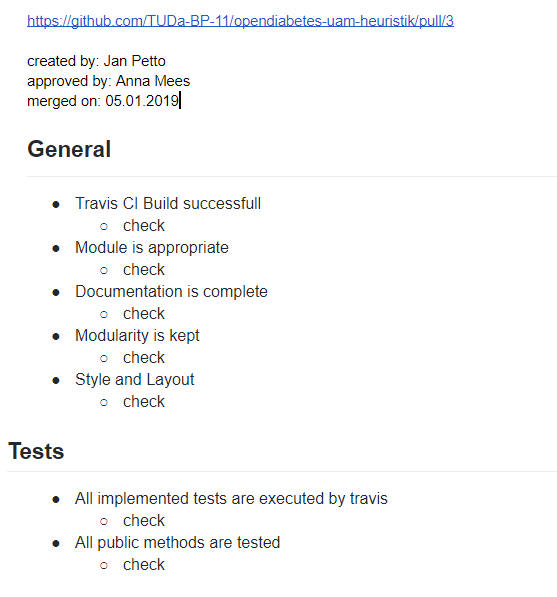
\includegraphics[width=\textwidth,height=\textheight,keepaspectratio]{pr-3}
\label{pr:3}
\end{figure}

\begin{figure}[h]
\centering
\caption{Pull Request \#4}
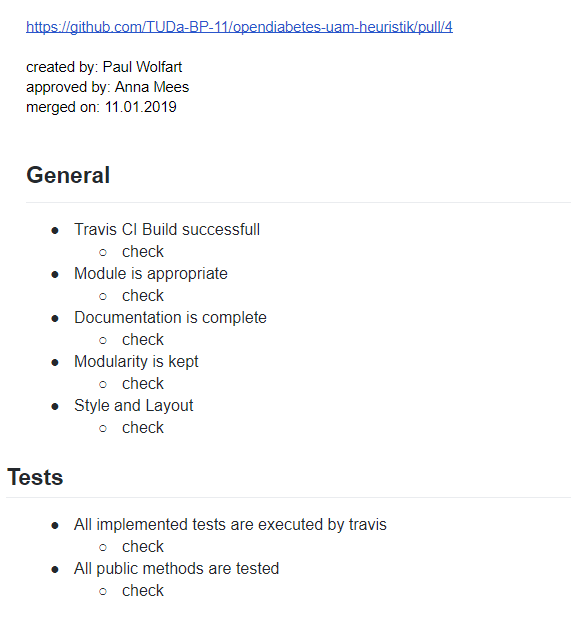
\includegraphics[width=\textwidth,height=\textheight,keepaspectratio]{pr-4}
\label{pr:4}
\end{figure}

\begin{figure}[h]
\centering
\caption{Pull Request \#13}
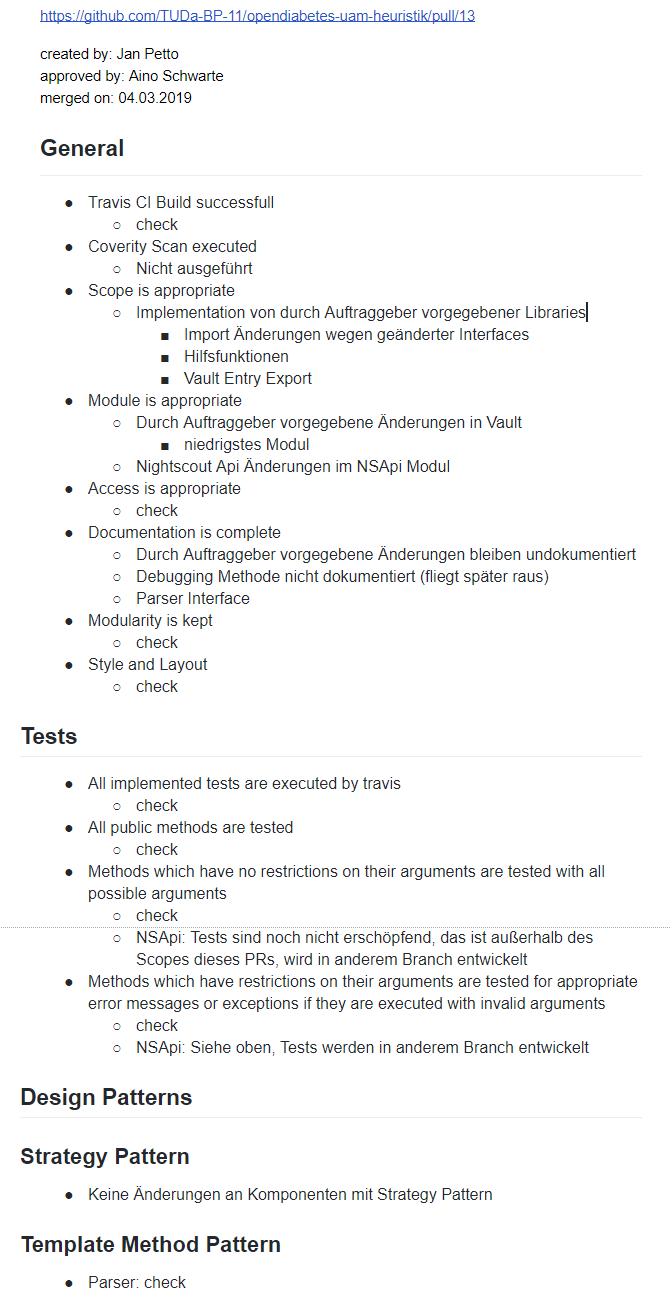
\includegraphics[width=\textwidth,height=\textheight,keepaspectratio]{pr-13}
\label{pr:13}
\end{figure}

\begin{figure}[h]
\centering
\caption{Test Coverage Pull Request \#13}
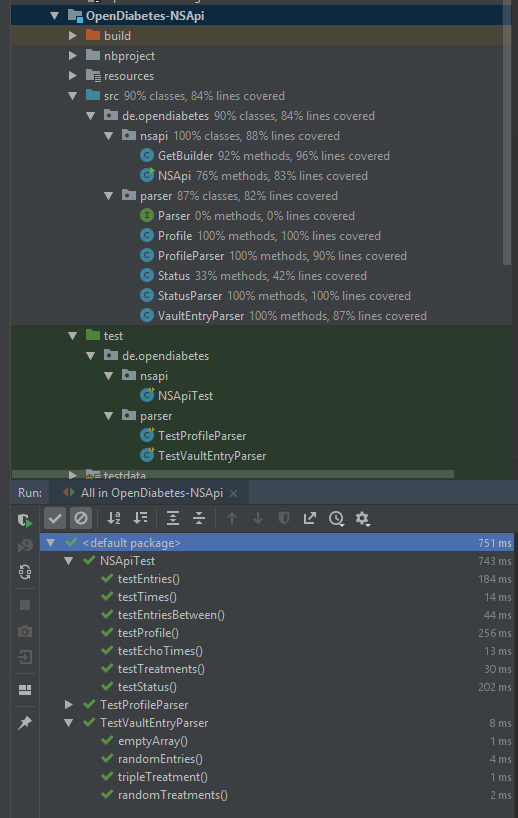
\includegraphics[width=\textwidth,height=\textheight,keepaspectratio]{pr-cov-13}
\label{pr-cov:13}
\end{figure}

\begin{figure}[h]
\centering
\caption{Pull Request \#15}
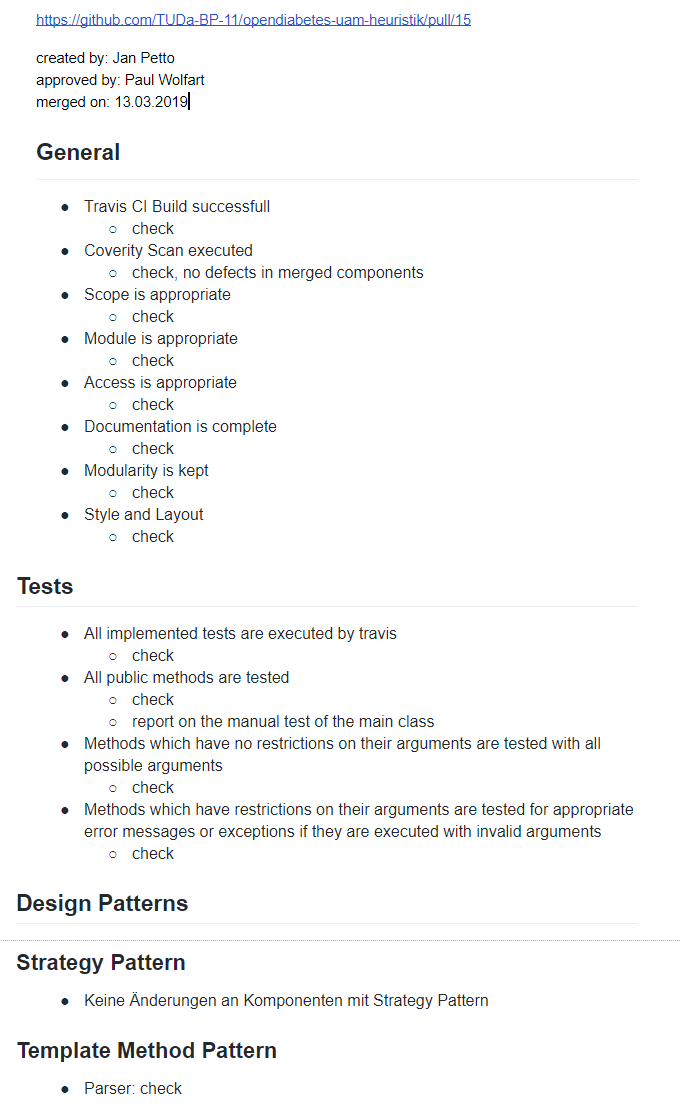
\includegraphics[width=\textwidth,height=\textheight,keepaspectratio]{pr-15}
\label{pr:15}
\end{figure}

\begin{figure}[h]
\centering
\caption{Test Coverage Pull Request \#15}
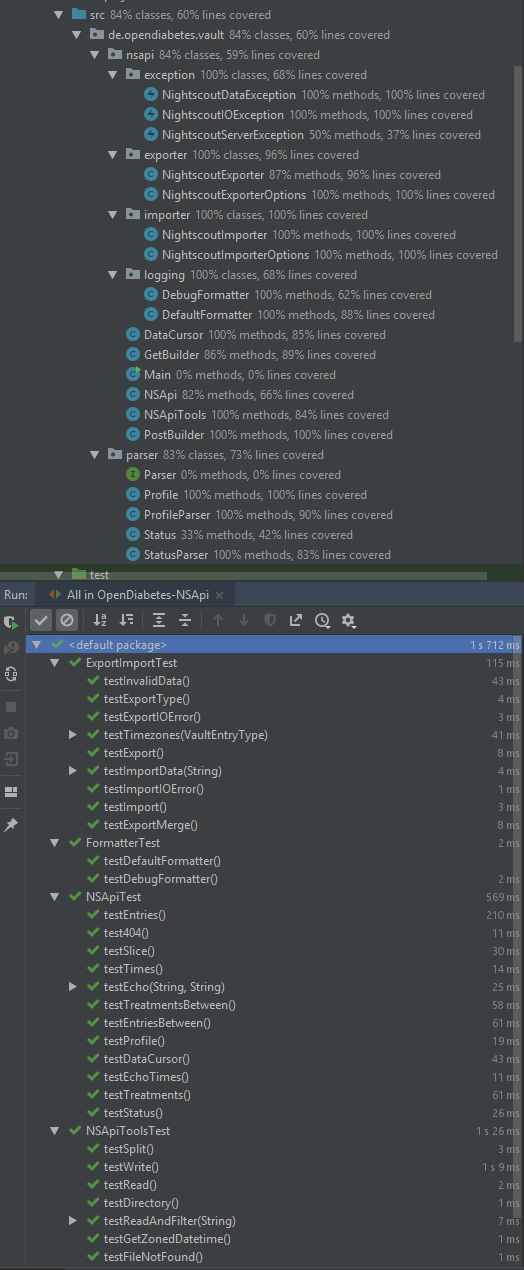
\includegraphics[width=\textwidth,height=\textheight,keepaspectratio]{pr-cov-15}
\label{pr-cov:15}
\end{figure}

\begin{figure}[h]
\centering
\caption{Manual Tests Pull Request \#15}
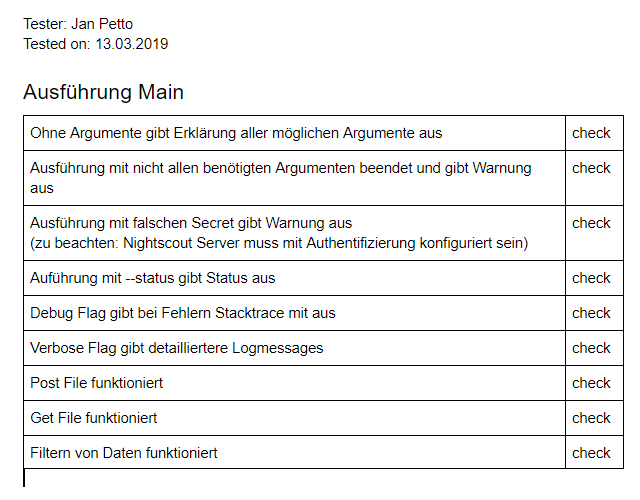
\includegraphics[width=\textwidth,height=\textheight,keepaspectratio]{pr-tests-15}
\label{pr-tests:15}
\end{figure}

\begin{figure}[h]
\centering
\caption{Pull Request \#16}
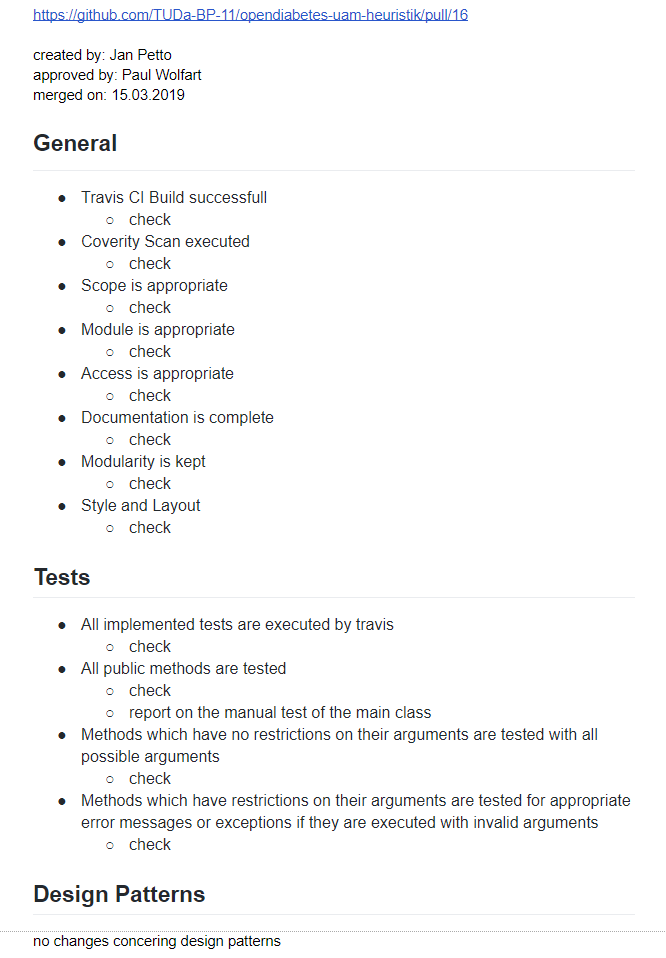
\includegraphics[width=\textwidth,height=\textheight,keepaspectratio]{pr-16}
\label{pr:16}
\end{figure}

\begin{figure}[h]
\centering
\caption{Test Coverage Pull Request \#16}
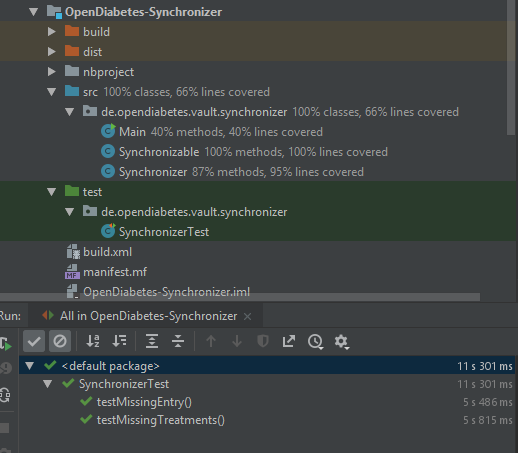
\includegraphics[width=\textwidth,height=\textheight,keepaspectratio]{pr-cov-16}
\label{pr-cov:16}
\end{figure}

\begin{figure}[h]
\centering
\caption{Manual Tests Pull Request \#16}
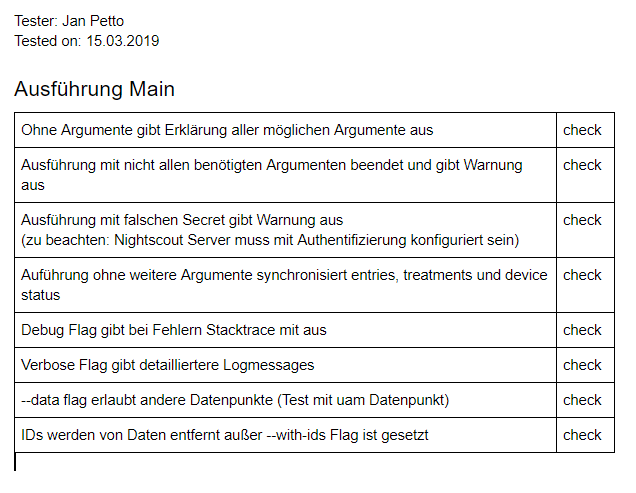
\includegraphics[width=\textwidth,height=\textheight,keepaspectratio]{pr-tests-16}
\label{pr-tests:16}
\end{figure}

\begin{figure}[h]
\centering
\caption{Pull Request \#18}
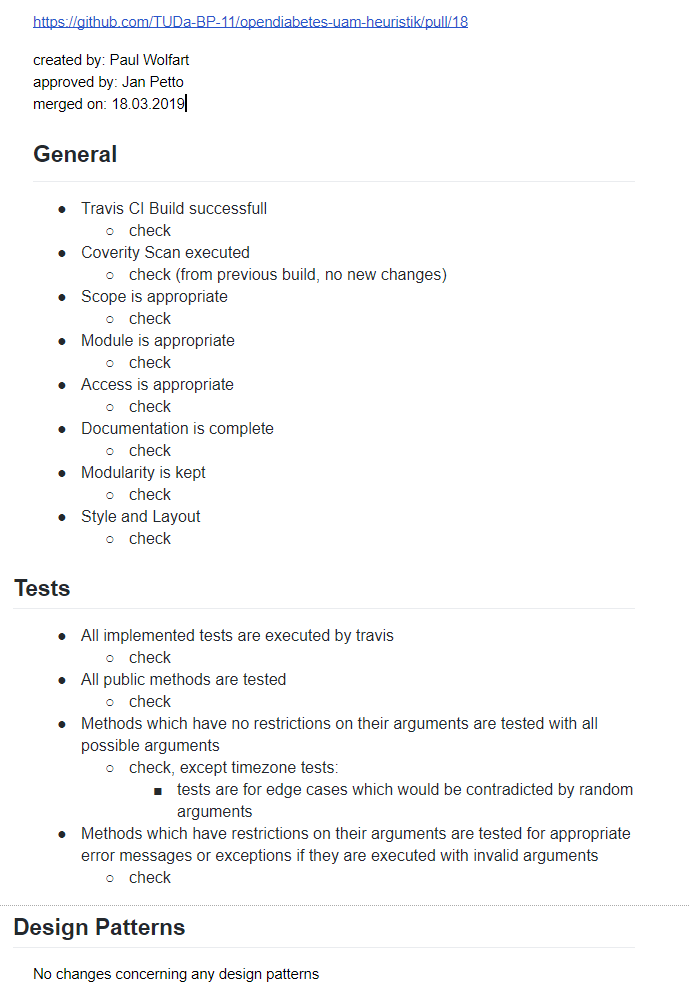
\includegraphics[width=\textwidth,height=\textheight,keepaspectratio]{pr-18}
\label{pr:18}
\end{figure}

\begin{figure}[h]
\centering
\caption{Test Coverage Pull Request \#18}
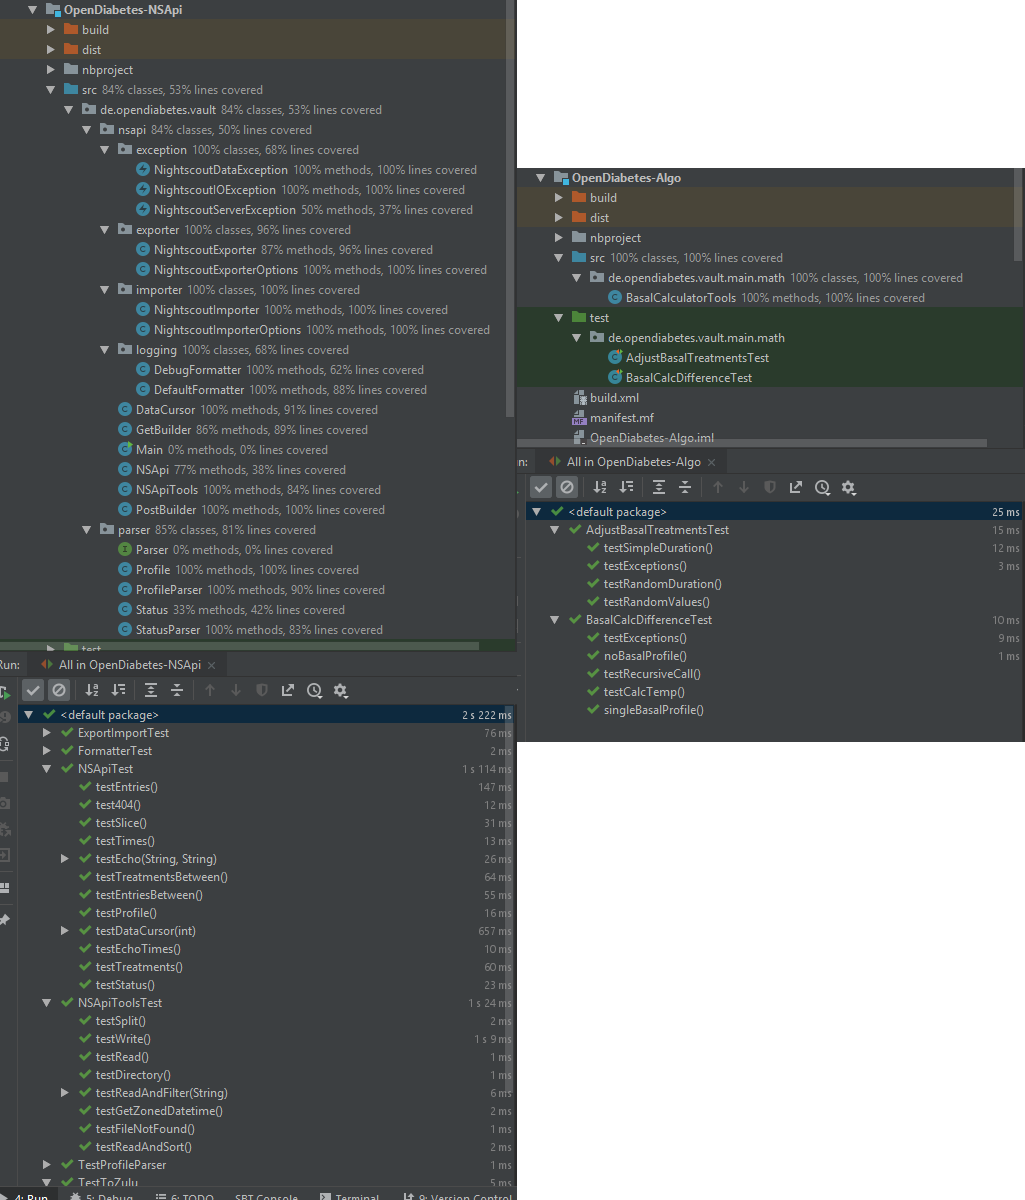
\includegraphics[width=\textwidth,height=\textheight,keepaspectratio]{pr-cov-18}
\label{pr-cov:18}
\end{figure}

\begin{figure}[h]
\centering
\caption{Pull Request \#45}
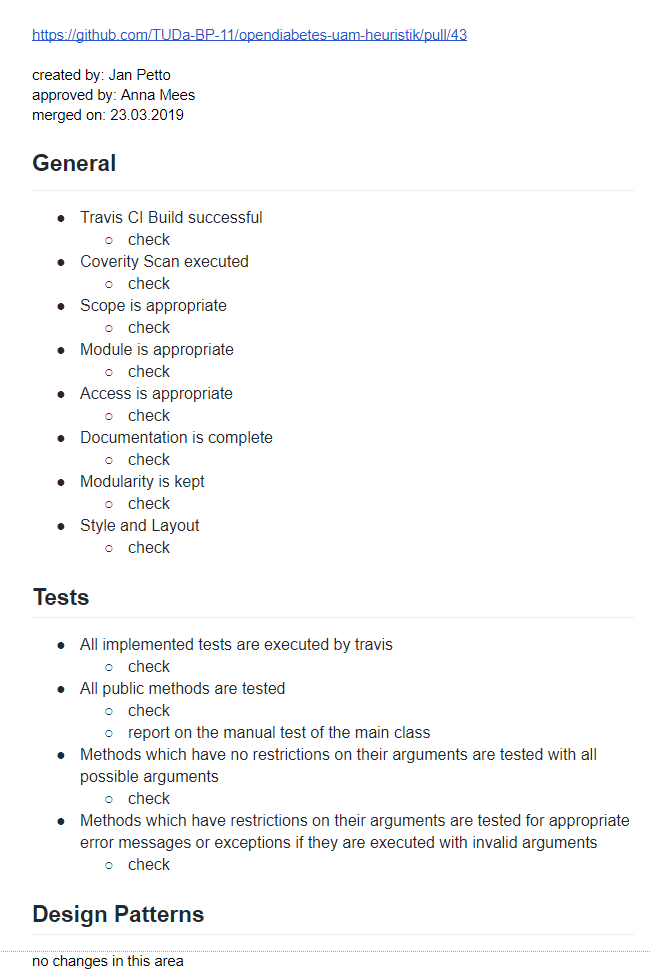
\includegraphics[width=\textwidth,height=\textheight,keepaspectratio]{pr-45}
\label{pr:45}
\end{figure}

\begin{figure}[h]
\centering
\caption{Pull Request \#43}
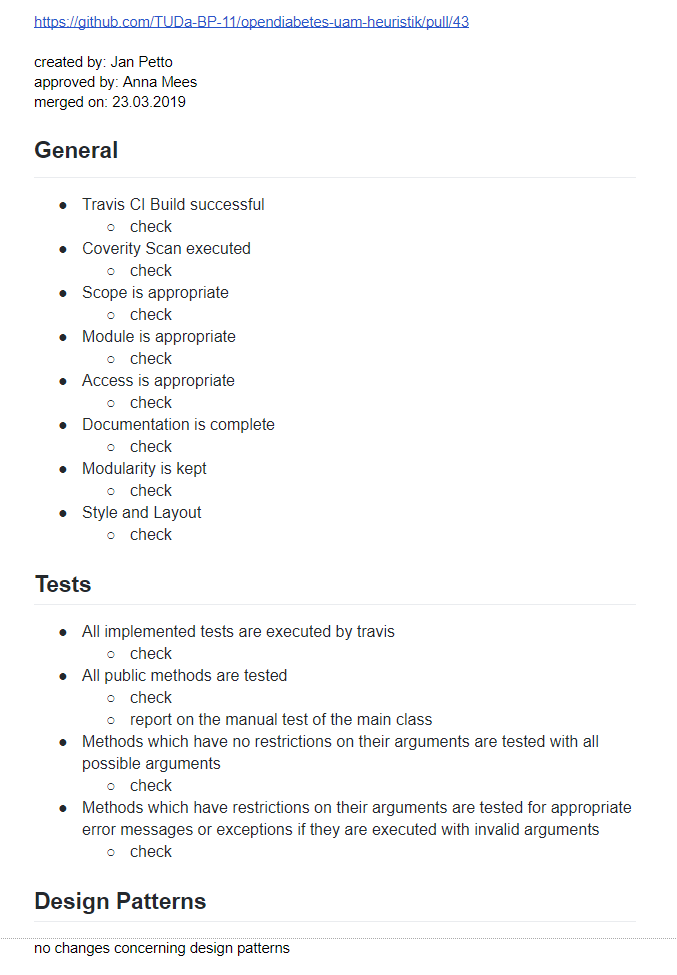
\includegraphics[width=\textwidth,height=\textheight,keepaspectratio]{pr-43}
\label{pr:43}
\end{figure}

\begin{figure}[h]
\centering
\caption{Test Coverage Pull Request \#43}
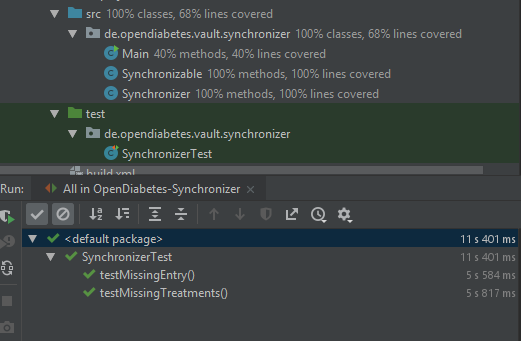
\includegraphics[width=\textwidth,height=\textheight,keepaspectratio]{pr-cov-43}
\label{pr-cov:43}
\end{figure}

\begin{figure}[h]
\centering
\caption{Manual Tests Pull Request \#43}
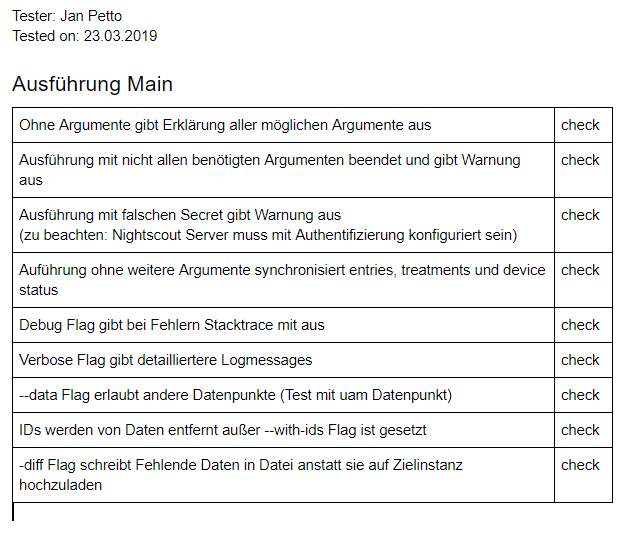
\includegraphics[width=\textwidth,height=\textheight,keepaspectratio]{pr-tests-43}
\label{pr-tests:43}
\end{figure}

\begin{figure}[h]
\centering
\caption{Pull Request \#46}
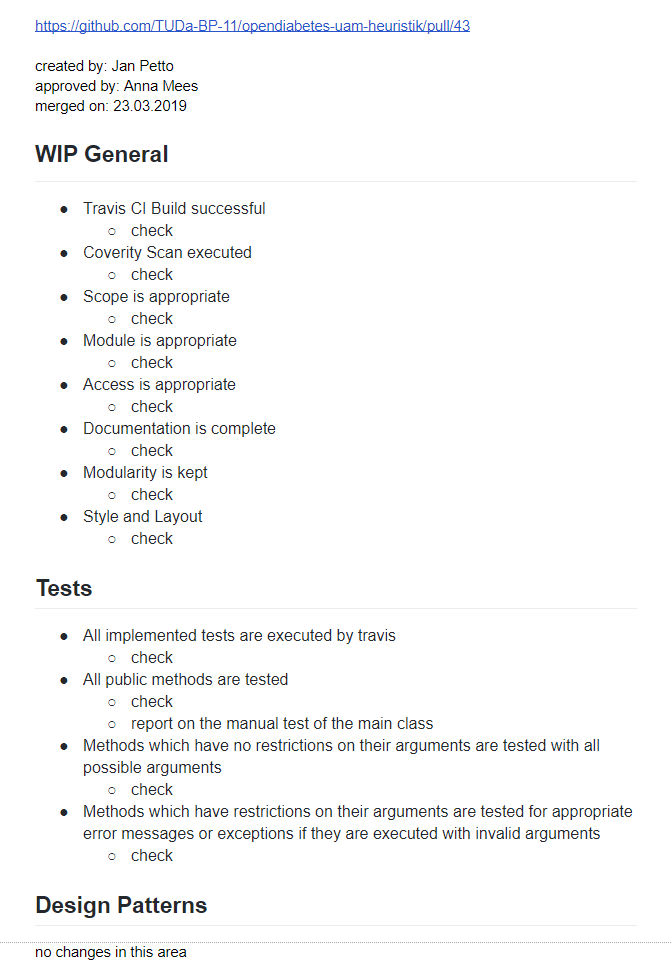
\includegraphics[width=\textwidth,height=\textheight,keepaspectratio]{pr-46}
\label{pr:46}
\end{figure}

\begin{figure}[h]
\centering
\caption{Pull Request \#52}

\includegraphics[width=\textwidth,height=\textheight,keepaspectratio]{pr-52}
\label{pr:52}
\end{figure}

\begin{figure}[h]
\centering
\caption{Pull Request \#47}
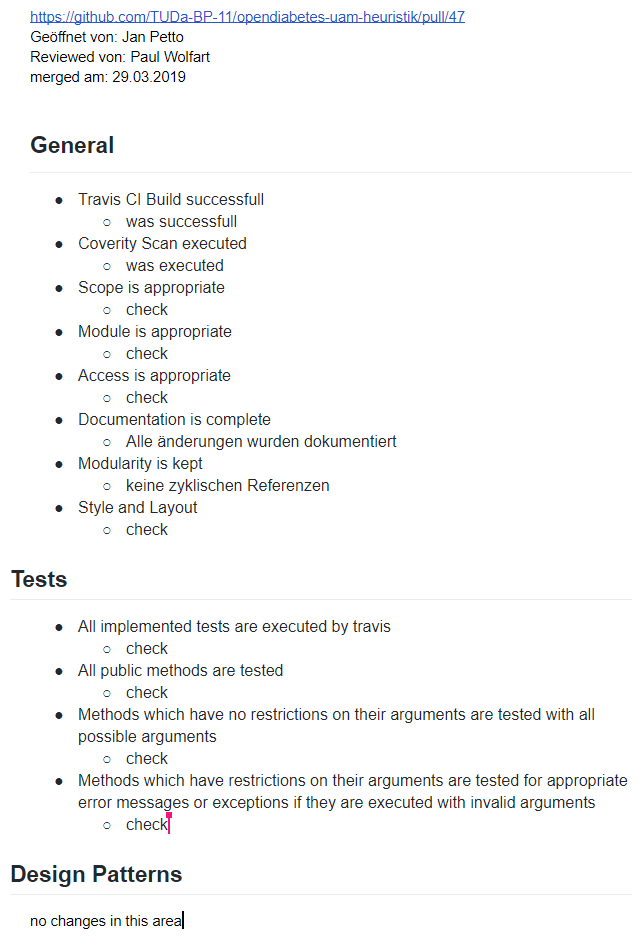
\includegraphics[width=\textwidth,height=\textheight,keepaspectratio]{pr-47}
\label{pr:47}
\end{figure}

\begin{figure}[h]
\centering
\caption{Test Coverage Pull Request \#47}
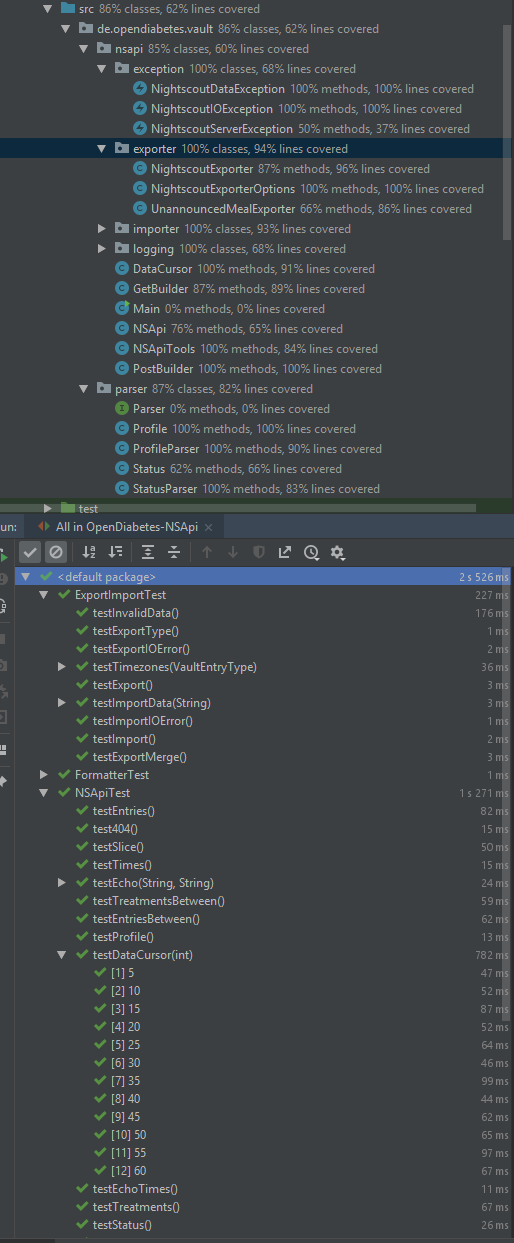
\includegraphics[width=\textwidth,height=\textheight,keepaspectratio]{pr-cov-47}
\label{pr-cov:47}
\end{figure}

\begin{figure}[h]
\centering
\caption{Pull Request \#51}
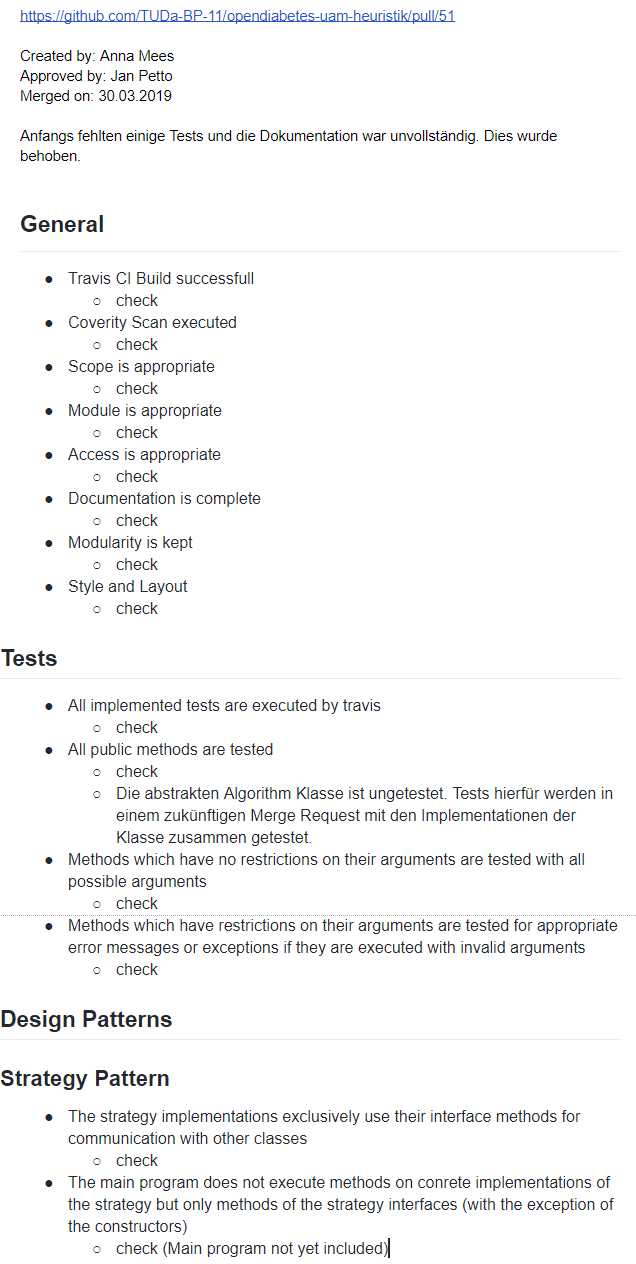
\includegraphics[width=\textwidth,height=\textheight,keepaspectratio]{pr-51}
\label{pr:51}
\end{figure}

\begin{figure}[h]
\centering
\caption{Test Coverage Pull Request \#51}
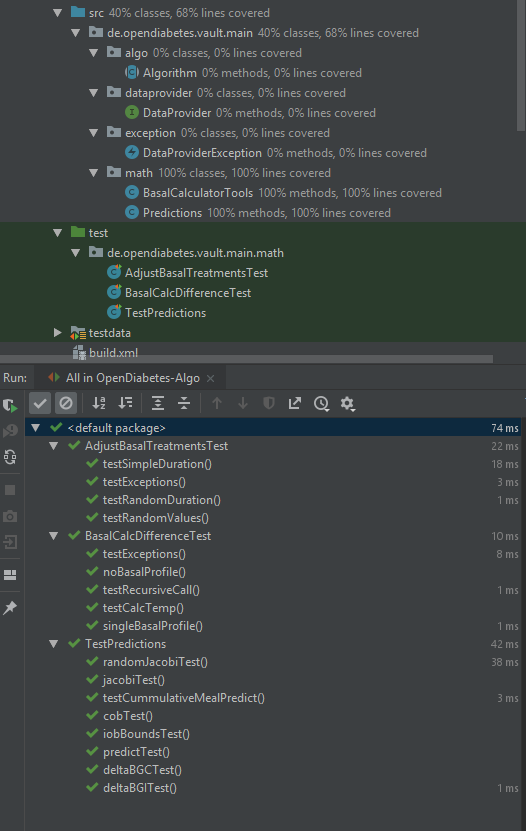
\includegraphics[width=\textwidth,height=\textheight,keepaspectratio]{pr-cov-51}
\label{pr-cov:51}
\end{figure}

\begin{figure}[h]
\centering
\caption{Pull Request \#54}
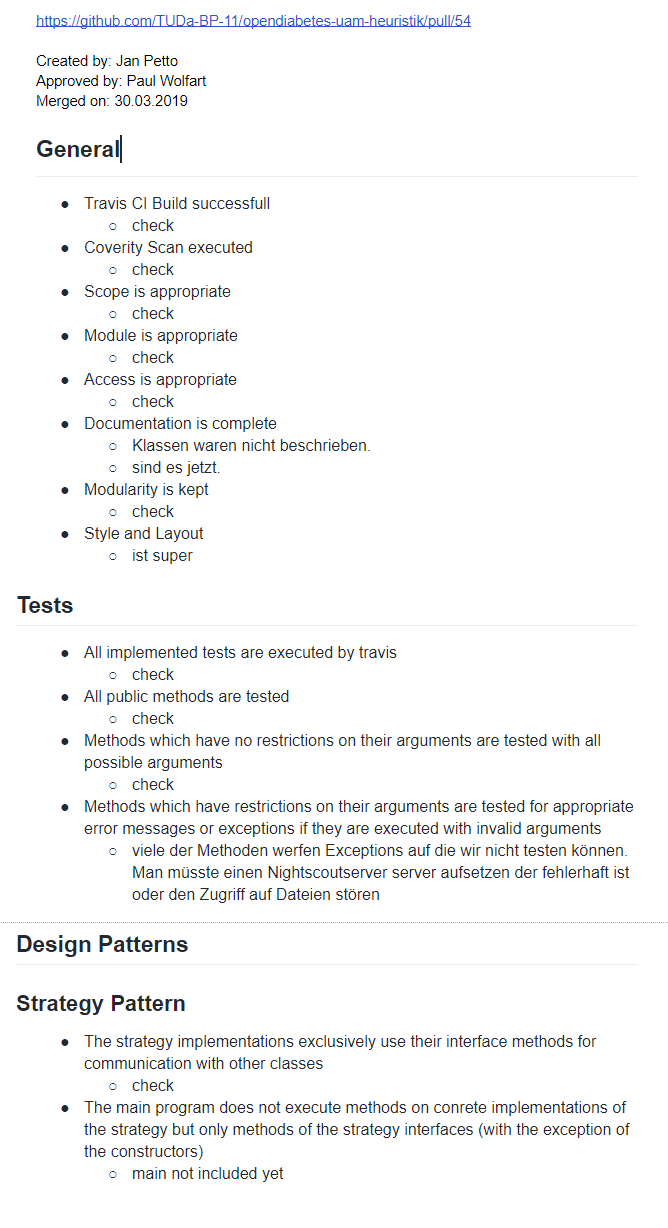
\includegraphics[width=\textwidth,height=\textheight,keepaspectratio]{pr-54}
\label{pr:54}
\end{figure}

\begin{figure}[h]
\centering
\caption{Test Coverage Pull Request \#54}
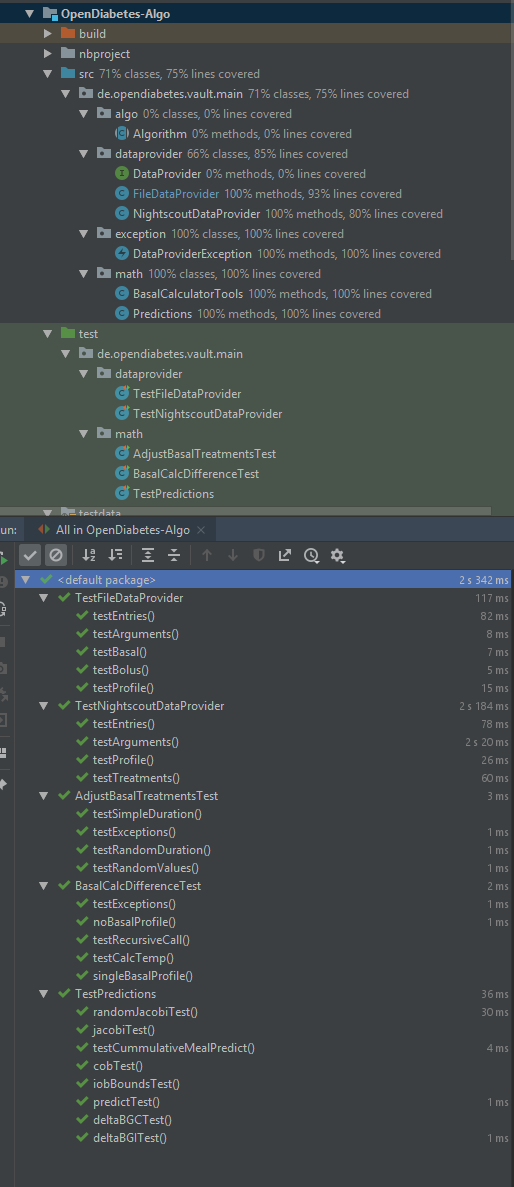
\includegraphics[width=\textwidth,height=\textheight,keepaspectratio]{pr-cov-54}
\label{pr-cov:54}
\end{figure}
	
\section{GitHub Wiki Artikel Checkliste}
\begin{itemize}
\item Alle Seiten sind in korrekter englischer Sprache verfasst
\item Am Anfang befindet sich eine Einleitung, die in das Projekt einführt
\item Jede Seite besitzt eine Table of Content
\item Anleitungen müssen vollständig und nachvollziehbar sein
	\begin{itemize}
	\item Befolgen der Anleitung muss zu dem gewünschten Ergebnis führen
	\end{itemize}
\item Alle relevanten Argumente/Spezifikationen müssen angegeben und erklärt sein
\item Zu jeder Erklärung muss es ein Beispiel geben
\item Leiten Verlinkungen zu den gewünschten Stellen korrekt weiter
\item Jedes Feature hat seine eigene Seite im Wiki
\item Jedes Feature wird am Anfang seiner Seite kurz erklärt
\end{itemize}


\section{GitHub Wiki Artikel Protokoll}

\paragraph{Home}
\begin{itemize}
\item Protokoll: Bild~\ref{wiki1}
\end{itemize}

\paragraph{Algorithm}
\begin{itemize}
\item Protokoll: abgelehnt Bild~\ref{wiki2}
\item Protokoll: Bild~\ref{wiki3}
\end{itemize}

\paragraph{Calculating unannounced meals}
\begin{itemize}
\item Protokoll: abgelehnt Bild~\ref{wiki4}
\item Protokoll: Bild~\ref{wiki5}
\end{itemize}

\paragraph{Checklist Pull Request Review}
\begin{itemize}
\item Protokoll: Bild~\ref{wiki6}
\end{itemize}

\paragraph{Implementing a new algorithm}
\begin{itemize}
\item Protokoll: abgelehnt Bild~\ref{wiki7}
\item Protokoll: Bild~\ref{wiki8}
\end{itemize}

\paragraph{Implementing a new data provider}
\begin{itemize}
\item Protokoll: abgelehnt Bild~\ref{wiki9}
\item Protokoll: Bild~\ref{wiki10}
\end{itemize}

\paragraph{Mapping Nightscout Data on to VaultEntry data}
\begin{itemize}
\item Protokoll: abgelehnt Bild~\ref{wiki11}
\item Protokoll: Bild~\ref{wiki12}
\end{itemize}

\paragraph{Nightscout API}
\begin{itemize}
\item Protokoll: Bild~\ref{wiki13}
\end{itemize}

\paragraph{Setting up a local Nightscout Server}
\begin{itemize}
\item Protokoll: Bild~\ref{wiki14}
\end{itemize}

\paragraph{Synchronizer}
\begin{itemize}
\item Protokoll: Bild~\ref{wiki15}
\end{itemize}



\begin{figure}[h]
\centering
\caption{Home}
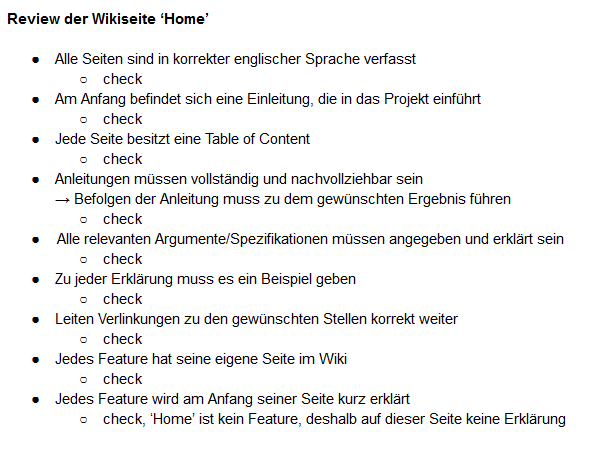
\includegraphics[width=0.8\textwidth]{wiki1}
\label{wiki1}
\end{figure}

\begin{figure}[h]
\centering
\caption{Algorithm, abgelehnt}
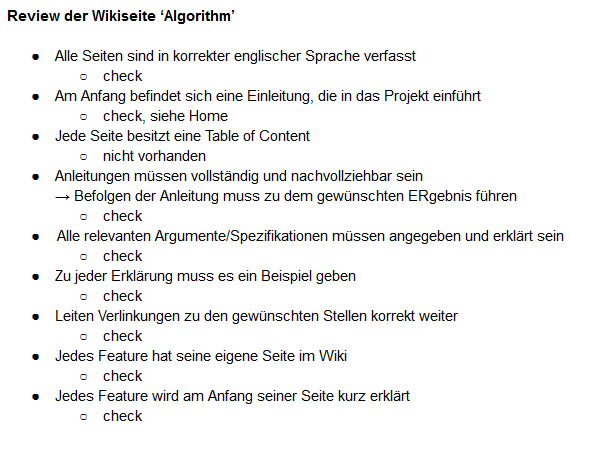
\includegraphics[width=0.8\textwidth]{wiki2}
\label{wiki2}
\end{figure}

\begin{figure}[h]
\centering
\caption{Algorithm}
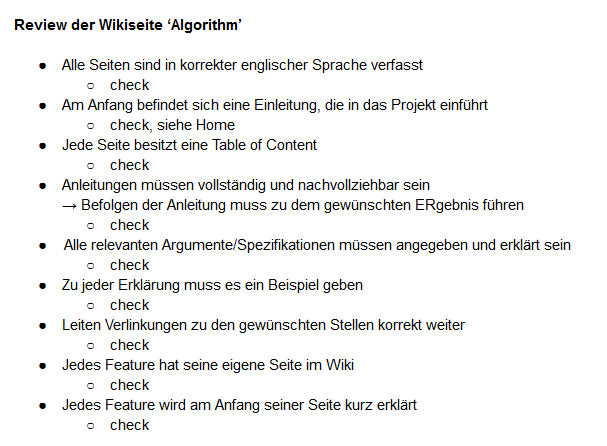
\includegraphics[width=0.8\textwidth]{wiki3}
\label{wiki3}
\end{figure}

\begin{figure}[h]
\centering
\caption{Calculating unannounced meals, abgelehnt}
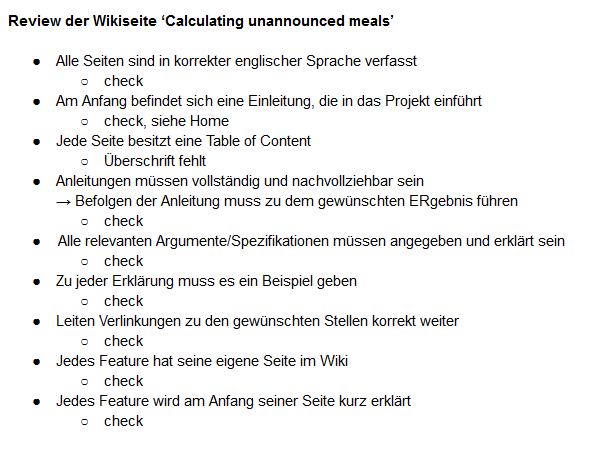
\includegraphics[width=0.8\textwidth]{wiki4}
\label{wiki4}
\end{figure}

\begin{figure}[h]
\centering
\caption{Calculating unannounced meals}
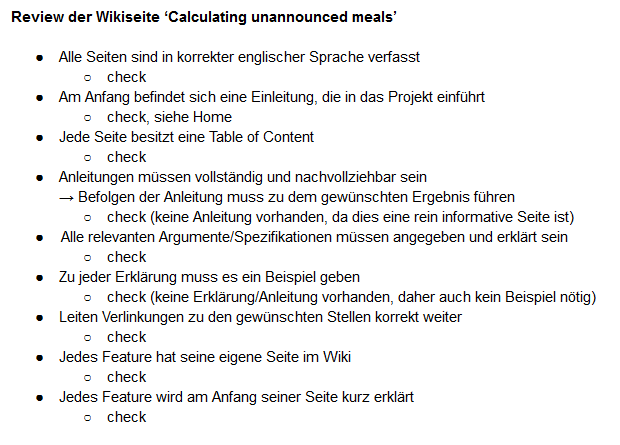
\includegraphics[width=0.8\textwidth]{wiki5}
\label{wiki5}
\end{figure}

\begin{figure}[h]
\centering
\caption{Checklist Pull Request Review}
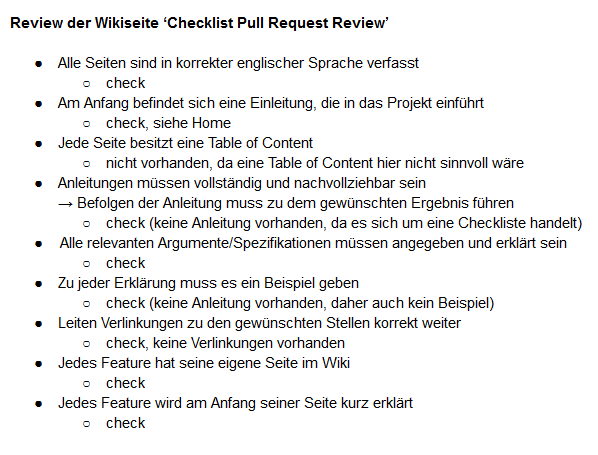
\includegraphics[width=0.8\textwidth]{wiki6}
\label{wiki6}
\end{figure}

\begin{figure}[h]
\centering
\caption{Implementing a new algorithm, abgelehnt}
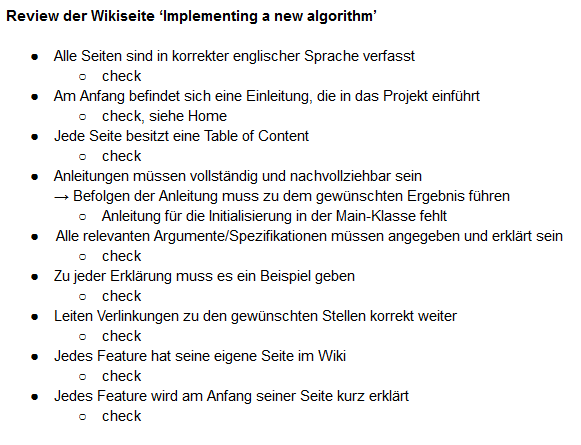
\includegraphics[width=0.8\textwidth]{wiki7}
\label{wiki7}
\end{figure}

\begin{figure}[h]
\centering
\caption{Implementing a new algorithm}
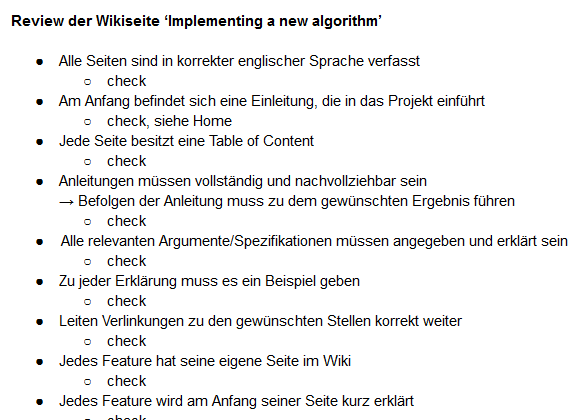
\includegraphics[width=0.8\textwidth]{wiki8}
\label{wiki8}
\end{figure}

\begin{figure}[h]
\centering
\caption{Implementing a new data provider, abgelehnt}
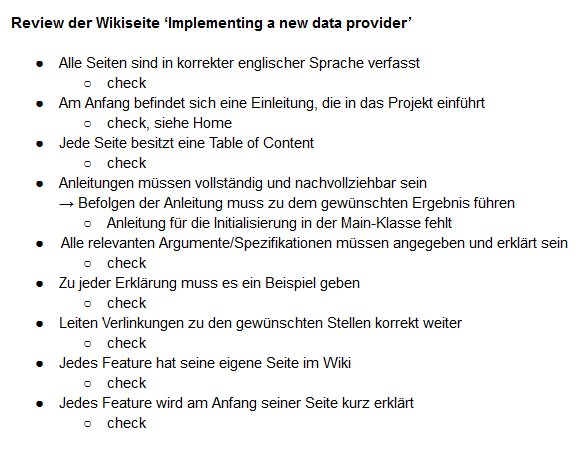
\includegraphics[width=0.8\textwidth]{wiki9}
\label{wiki9}
\end{figure}

\begin{figure}[h]
\centering
\caption{Implementing a new data provider}
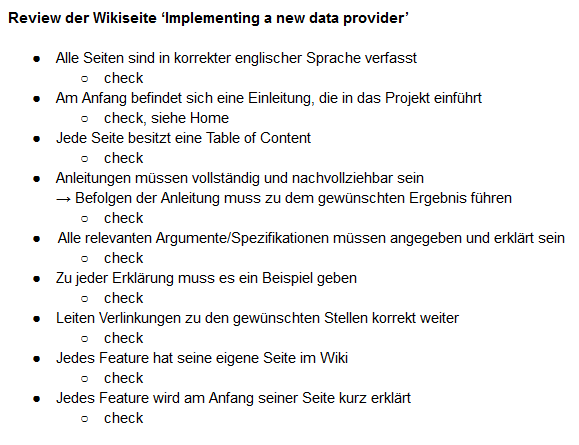
\includegraphics[width=0.8\textwidth]{wiki10}
\label{wiki10}
\end{figure}

\begin{figure}[h]
\centering
\caption{Mapping Nightscout Data on to VaultEntry data, abgelehnt}
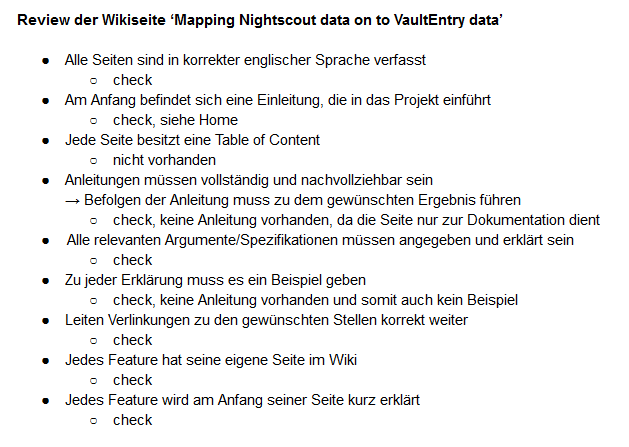
\includegraphics[width=0.8\textwidth]{wiki11}
\label{wiki11}
\end{figure}

\begin{figure}[h]
\centering
\caption{Mapping Nightscout Data on to VaultEntry data}
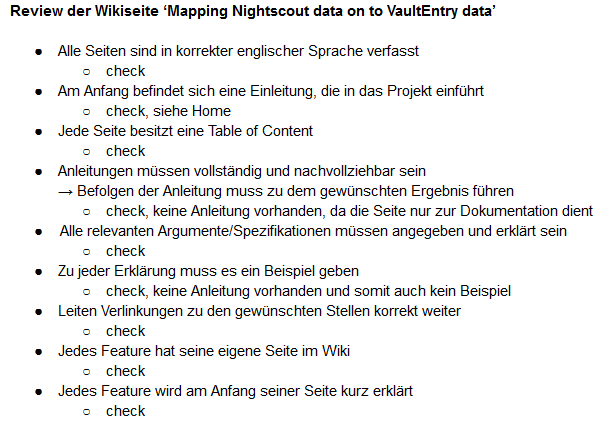
\includegraphics[width=0.8\textwidth]{wiki12}
\label{wiki12}
\end{figure}

\begin{figure}[h]
\centering
\caption{Nightscout API}
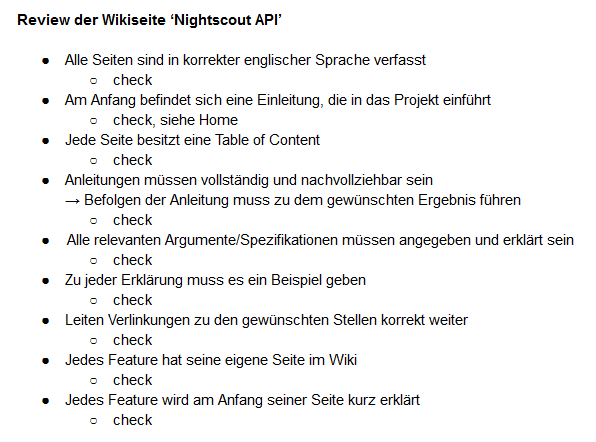
\includegraphics[width=0.8\textwidth]{wiki13}
\label{wiki13}
\end{figure}

\begin{figure}[h]
\centering
\caption{Setting up a local Nightscout Server}
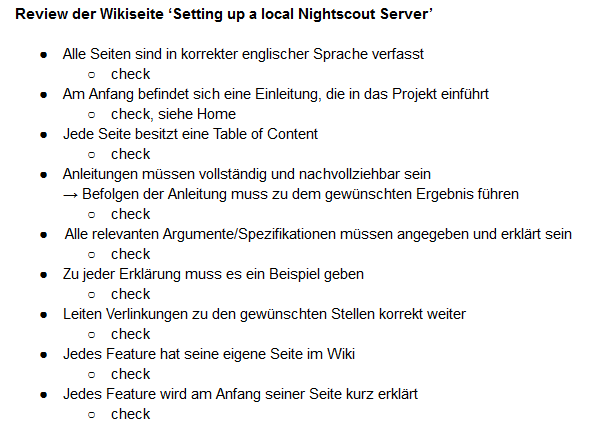
\includegraphics[width=0.8\textwidth]{wiki14}
\label{wiki14}
\end{figure}

\begin{figure}[h]
\centering
\caption{Synchronizer}
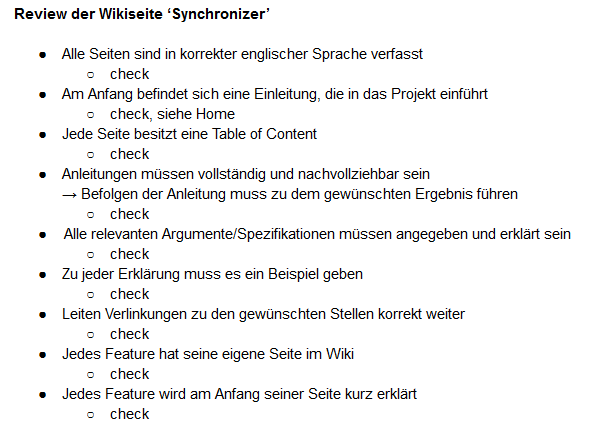
\includegraphics[width=0.8\textwidth]{wiki15}
\label{wiki15}
\end{figure}


\section{Tests}
\subsection{Unit Tests und Coverage}
Die vollständige Liste aller Tests ist in Bild~\ref{fig:all-tests} nachzuvollziehen.
Die Code-Coverage der Tests wurde zu unterschiedlichen Zeitpunkten aber insbesondere bei den verschiedenen Pull-Request-Reviews überprüft. Beispiele können in den folgenden Bildern nachvollzogen werden: \ref{pr-cov:13}, \ref{pr-cov:15}, \ref{pr-cov:16}, \ref{pr-cov:18}, \ref{pr-cov:18}, \ref{pr-cov:43}, \ref{pr-cov:47}, \ref{pr-cov:51}, \ref{pr-cov:54}

Ziel der Coverage war es für alle API-Methoden 100\% Methoden-Abdeckung zu erreichen. Nicht abgedeckte Zeilen sind vor allem \texttt{try-catch}-Blöcke für Sonderfälle wie unzeichende Dateizugriffs-Rechte, Serverprobleme etc. welche nicht zuverlässig mit Unit Tests testbar waren. Zusätzlich wurden die ,,Main'' Klassen und der Plotter nicht mit Unit Tests getestet sondern die funktionalen Anforderungen mit manuellen Tests überprüft.

\begin{figure}[h]
\centering
\caption{All Tests}
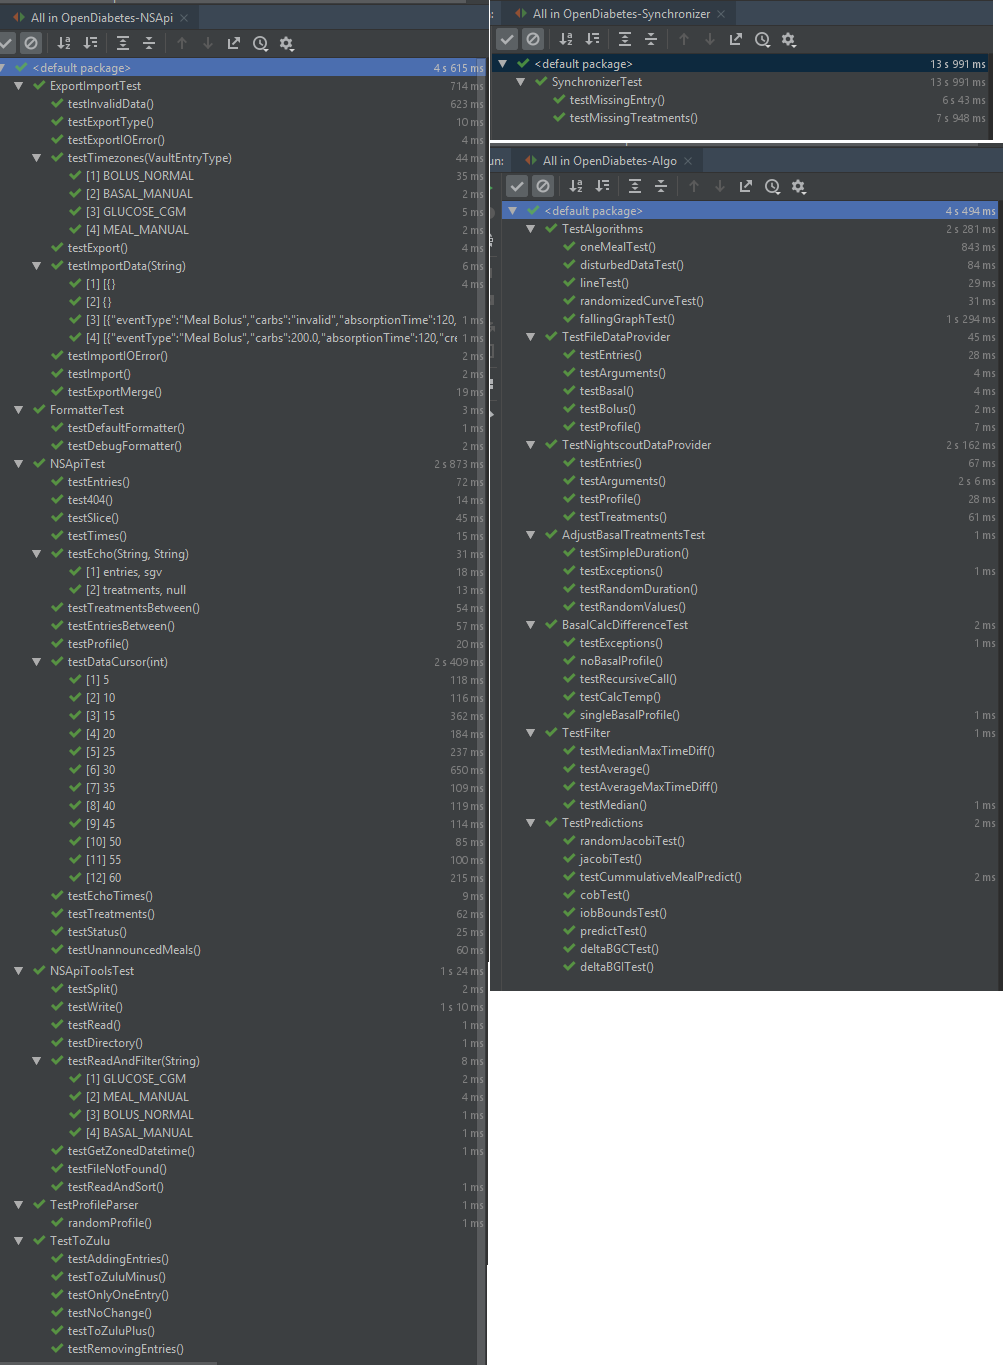
\includegraphics[width=\textwidth,height=\textheight,keepaspectratio]{all-tests}
\label{fig:all-tests}
\end{figure}

\subsection{Tests der Algorithmen}
Die Unit Tests der Algorithmen sind zur Beurteilung der Qualität der Algorithmen nicht sehr aussagekräftig, viel wichtiger war anhand von anonymisierten Daten zu ermitteln wie groß der jeweilige Fehler der errechneten Mahlzeiten und der daraus resultierenden Blutzuckerkurve ist. Die Fehlertoleranz hierfür wurde uns vom Auftraggeber vorgegeben (10\% Fehler über einen Zeitraum von sechs Stunden relativ zur echten Blutzuckerkurve). Diese Toleranz kann aber nicht für automatische Tests verwendet werden, da in den Testdaten sowohl Messfehler vorhanden sind, als auch größere Zeitsprünge, welche das Ergebnis verfälschen. Dies bedeutet dass Tests auf echten Daten immer manuell beurteilt werden mussten.

Anhand der entstandenen Statistiken konnten wir schnell beurteilen welche Ansätze vielversprechende Resultate bringen werden und welche Ansätze nicht weiter verfolgt werden mussten, da sie wahrscheinlich nie die geforderten Kriterien erfüllen würden. So hatte zum Beispiel die anfangs noch vielversprechende Idee, das Rauschen in den Daten mit einem Filter zu minimieren, im Endergebnis einen gegenteiligen Effekt.

Trotzdem wurde für sämtliche Schritte der den Algorithmen zu Grunde liegenden mathematischen Modelle Unit Tests geschrieben (Beispiel: TestPredictions.java \ref{lst:jacobi}).

\subsection{Test Beispiele}

\lstinputlisting[title=TestPredictions.java,label=lst:jacobi]{TestPredictions.java}

\lstinputlisting[title=NSApiTest.java]{NSApiTest.java}

\lstinputlisting[title=AdjustBasalTreatmentsTest.java]{AdjustBasalTreatmentsTest.java}

\lstinputlisting[title=BasalCalcDifferenceTest.java]{BasalCalcDifferenceTest.java}

\section{Code Beispiele}
\subsection{DataCursor}
Der \texttt{DataCursor} kann benutzt werden um durch Nightscout Daten zu iterieren. Der Cursor lädt die Daten dafür in einen internen Puffer, der automatisch aufgefüllt wird. Der Nightscout Server gibt Daten immer in absteigender Reihenfolge sortiert nach Datum zurück, weswegen der \texttt{DataCursor} von einem \texttt{latest} Zeitpunkt absteigend zu einem \texttt{oldest} Zeitpunkt durch die Daten iteriert. Alle Nightscout API Pfade, welche bei einem HTTP GET Request ein Array an Daten zurück geben, können benutzt werden, solange die zurückgegebenen Daten ein Datumsfeld beinhalten.
\lstinputlisting[title=DataCursor.java]{DataCursor.java}

\subsection{NightscoutImporter}
Der \texttt{NightscoutImporter} importiert Nightscout Daten und erzeugt eine Liste von \texttt{VaultEntry} Objekten. Er implementiert dabei die vom Auftraggeber vorgegebene \texttt{Importer} Klasse.
\lstinputlisting[title=NightscoutImporter.java]{NightscoutImporter.java}

\section{Coverity Scan}
Die Konfiguration von \href{https://scan.coverity.com/projects/tuda-bp-11-opendiabetes-uam-heuristik}{Coverity Scan} erwies sich als schwierig, denn es können zwar Pfade angeben werden, welche nicht getestet werden sollen, Änderungen an den Einstellungen lassen sich aber nicht speichern. In diversen Internetforen lässt sich beobachten, dass auch andere Benutzer das gleiche Problem haben, weswegen wir dazu übergegangen sind die Defekte aus dem Code unseres Auftragebers als ,,absichtlich'' zu markieren. Probleme in den Tests konnten in allen Fällen als ,,falsch-positiv'' oder ,,absichtlich'' markiert werden.\\
Die häufigsten ,,falsch-positiven'' Ereignisse waren String to Byte bzw. Byte to String Konvertierungen.
Die meisten Probleme die gefunden wurden waren Variablen und Felder die nicht benutzt oder nur aktualisiert wurden, danach waren es Felder und Methoden die nicht als statisch markiert wurden obwohl sie so benutzt wurden. Diese Probleme wurden behoben.

\subsection{Beispiel gefundener Bug}
\label{sec:coverity_bug}
In Bild~\ref{fig:coverity_bug} gibt die Funktion \texttt{getRawBasalTreatments()} null zurück und löst damit eine NullPointerException aus.

\begin{figure}[h]
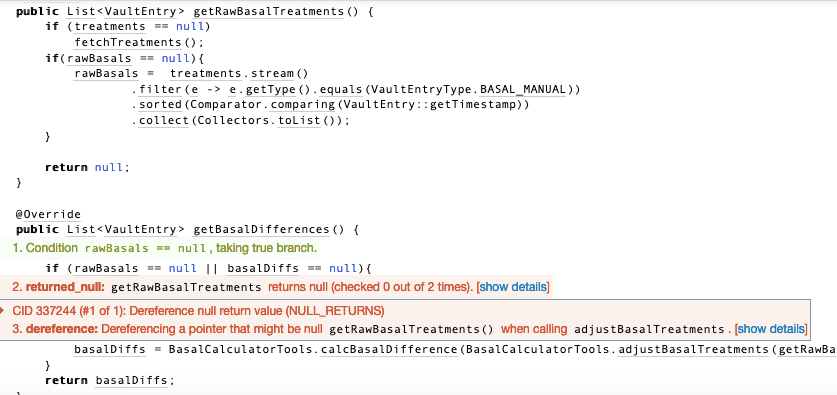
\includegraphics[width=1.0\textwidth]{Coverity_Bug}
\caption{NullPointerException Beispiel \ref{sec:coverity_bug}}
\centering
\label{fig:coverity_bug}
\end{figure}

\subsection{Beispiel False Positive}
\label{sec:coverity_fp}
In Bild~\ref{fig:coverity_fp1} wird \texttt{!allFilesSet(config)} zu false ausgewertet.
\\
In Bild~\ref{fig:coverity_fp2} wird das Inverse, also \texttt{allFilesSet(config)} auch zu false ausgewertet.

\begin{figure}[h]
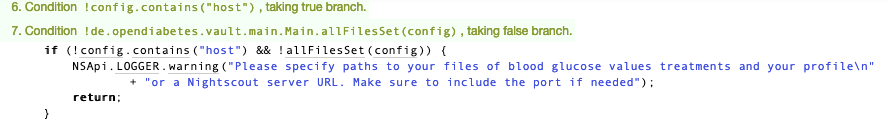
\includegraphics[width=1.0\textwidth]{Coverity_FP1}
\caption{False Positive Beispiel \ref{sec:coverity_fp}}
\centering
\label{fig:coverity_fp1}
\end{figure}

\newpage

\begin{figure}[h]
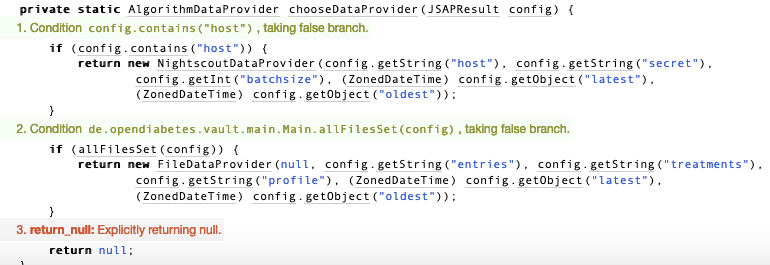
\includegraphics[width=1.0\textwidth]{Coverity_FP2}
\caption{False Positive Beispiel \ref{sec:coverity_fp}}
\centering
\label{fig:coverity_fp2}
\end{figure}


\section{Build Logs Beispiele}

\subsection{Build PR45 failed}

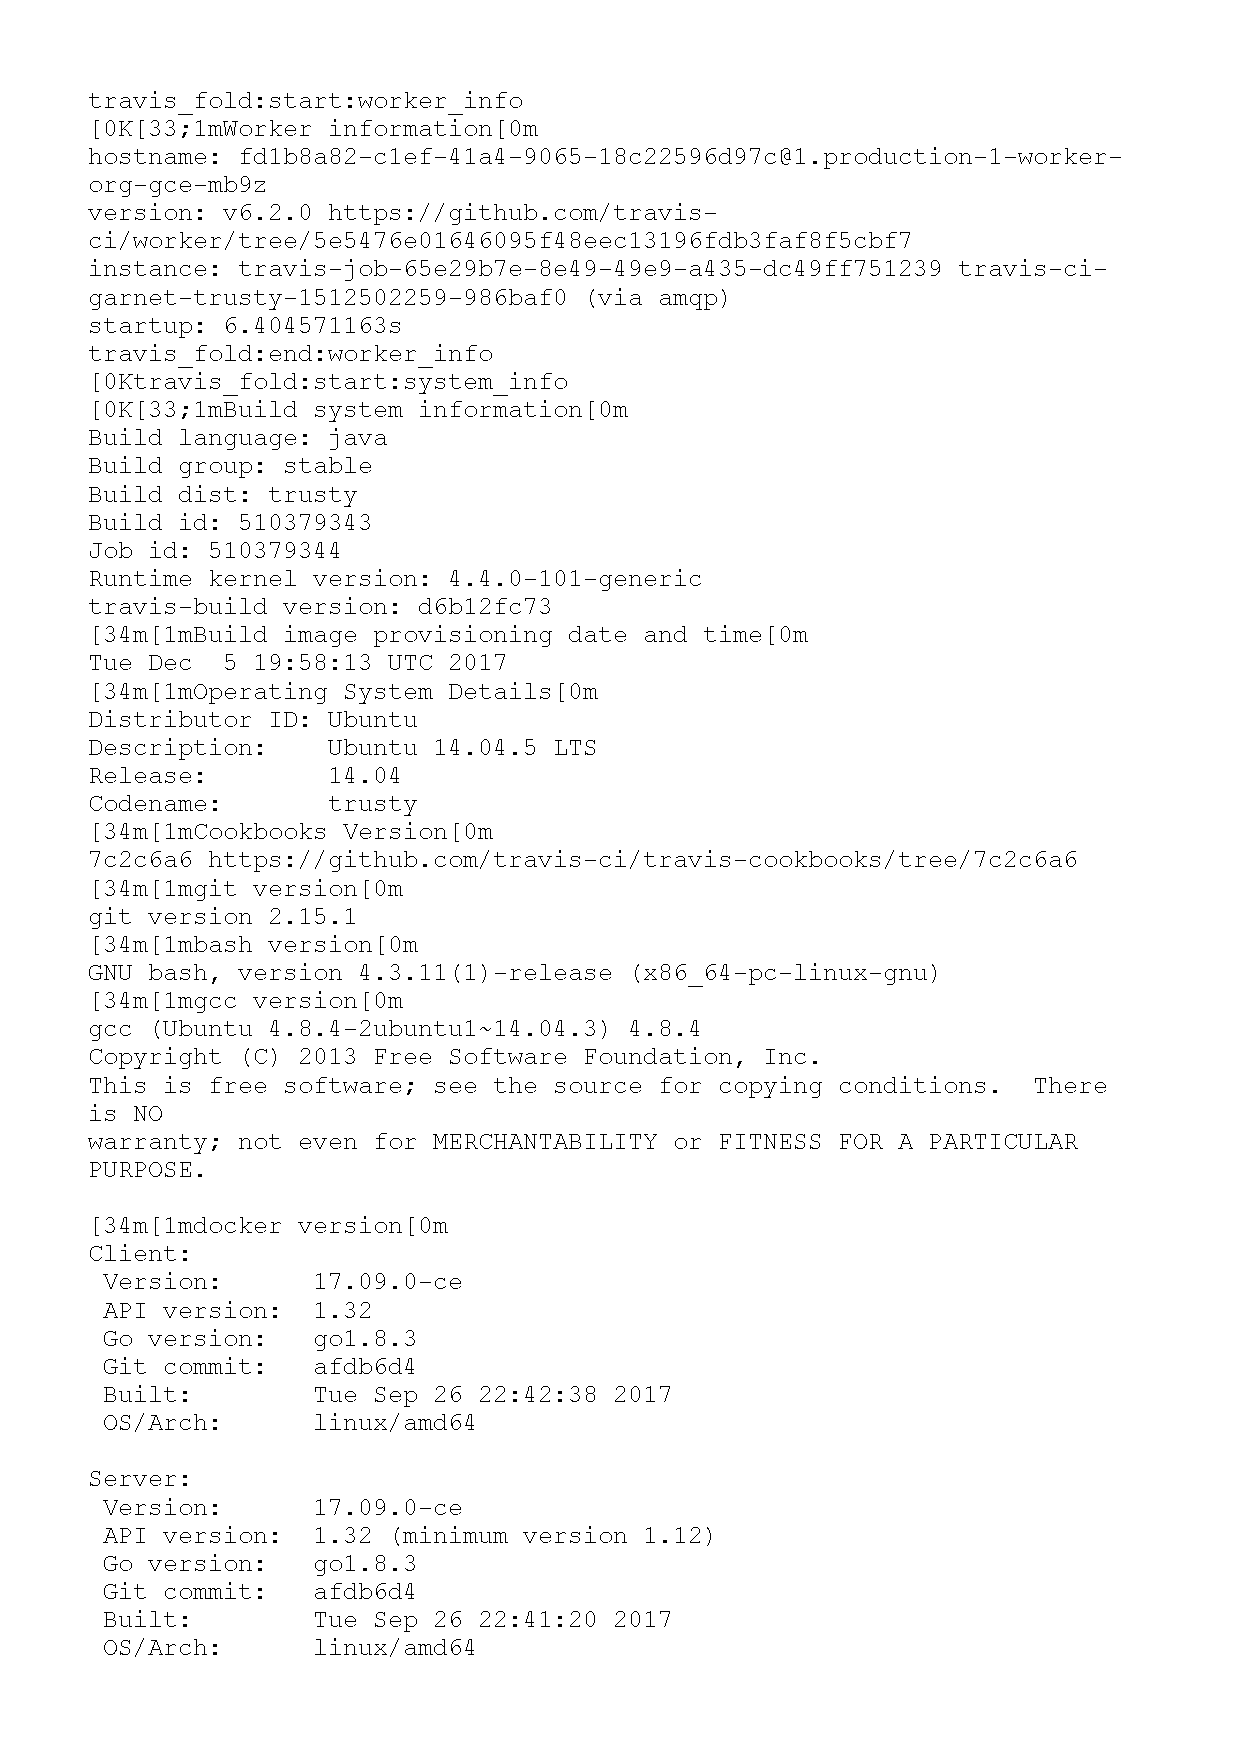
\includepdf[pages=-,scale=.9]{Build_PR45_failed.pdf}

\subsection{Build PR45 passed}

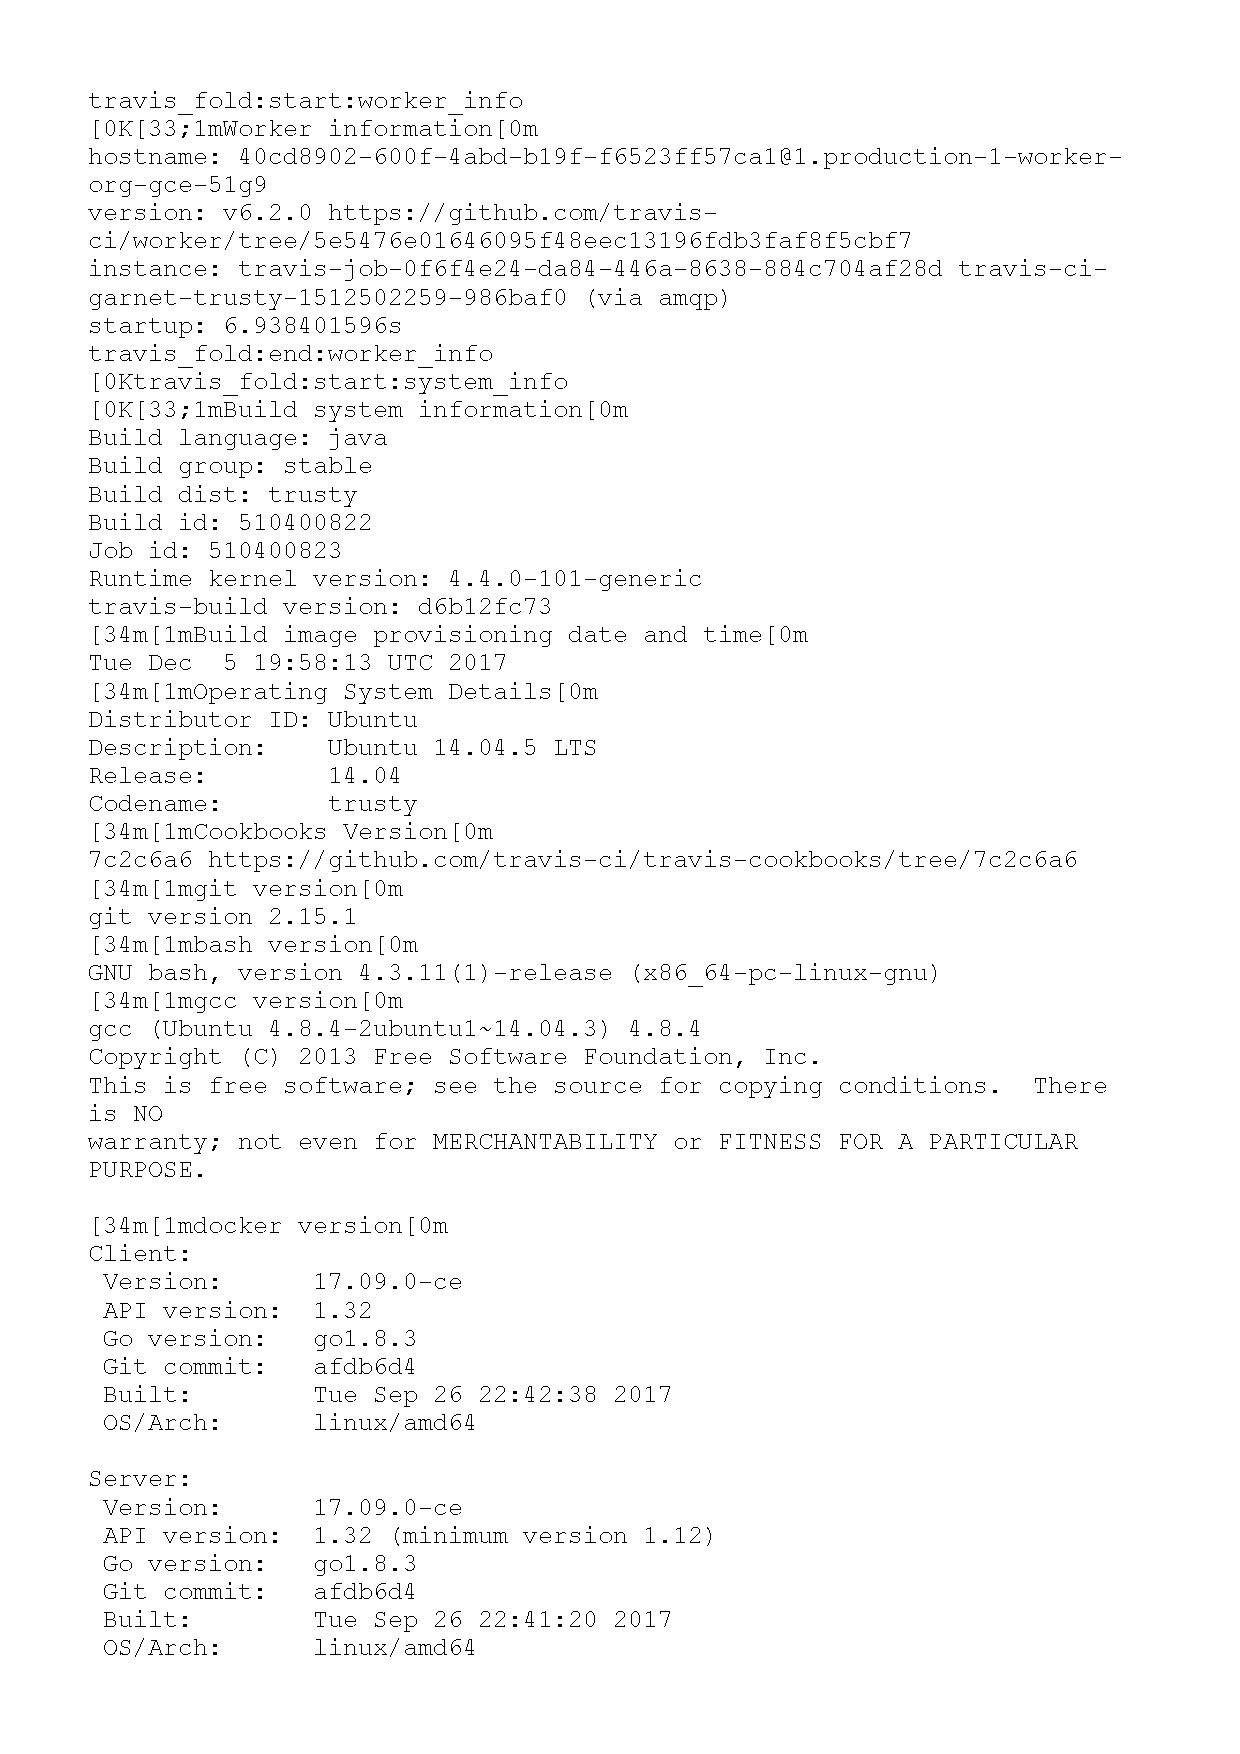
\includepdf[pages=-,scale=.9]{Build_PR45_passed.pdf}

\subsection{Build453 failed}

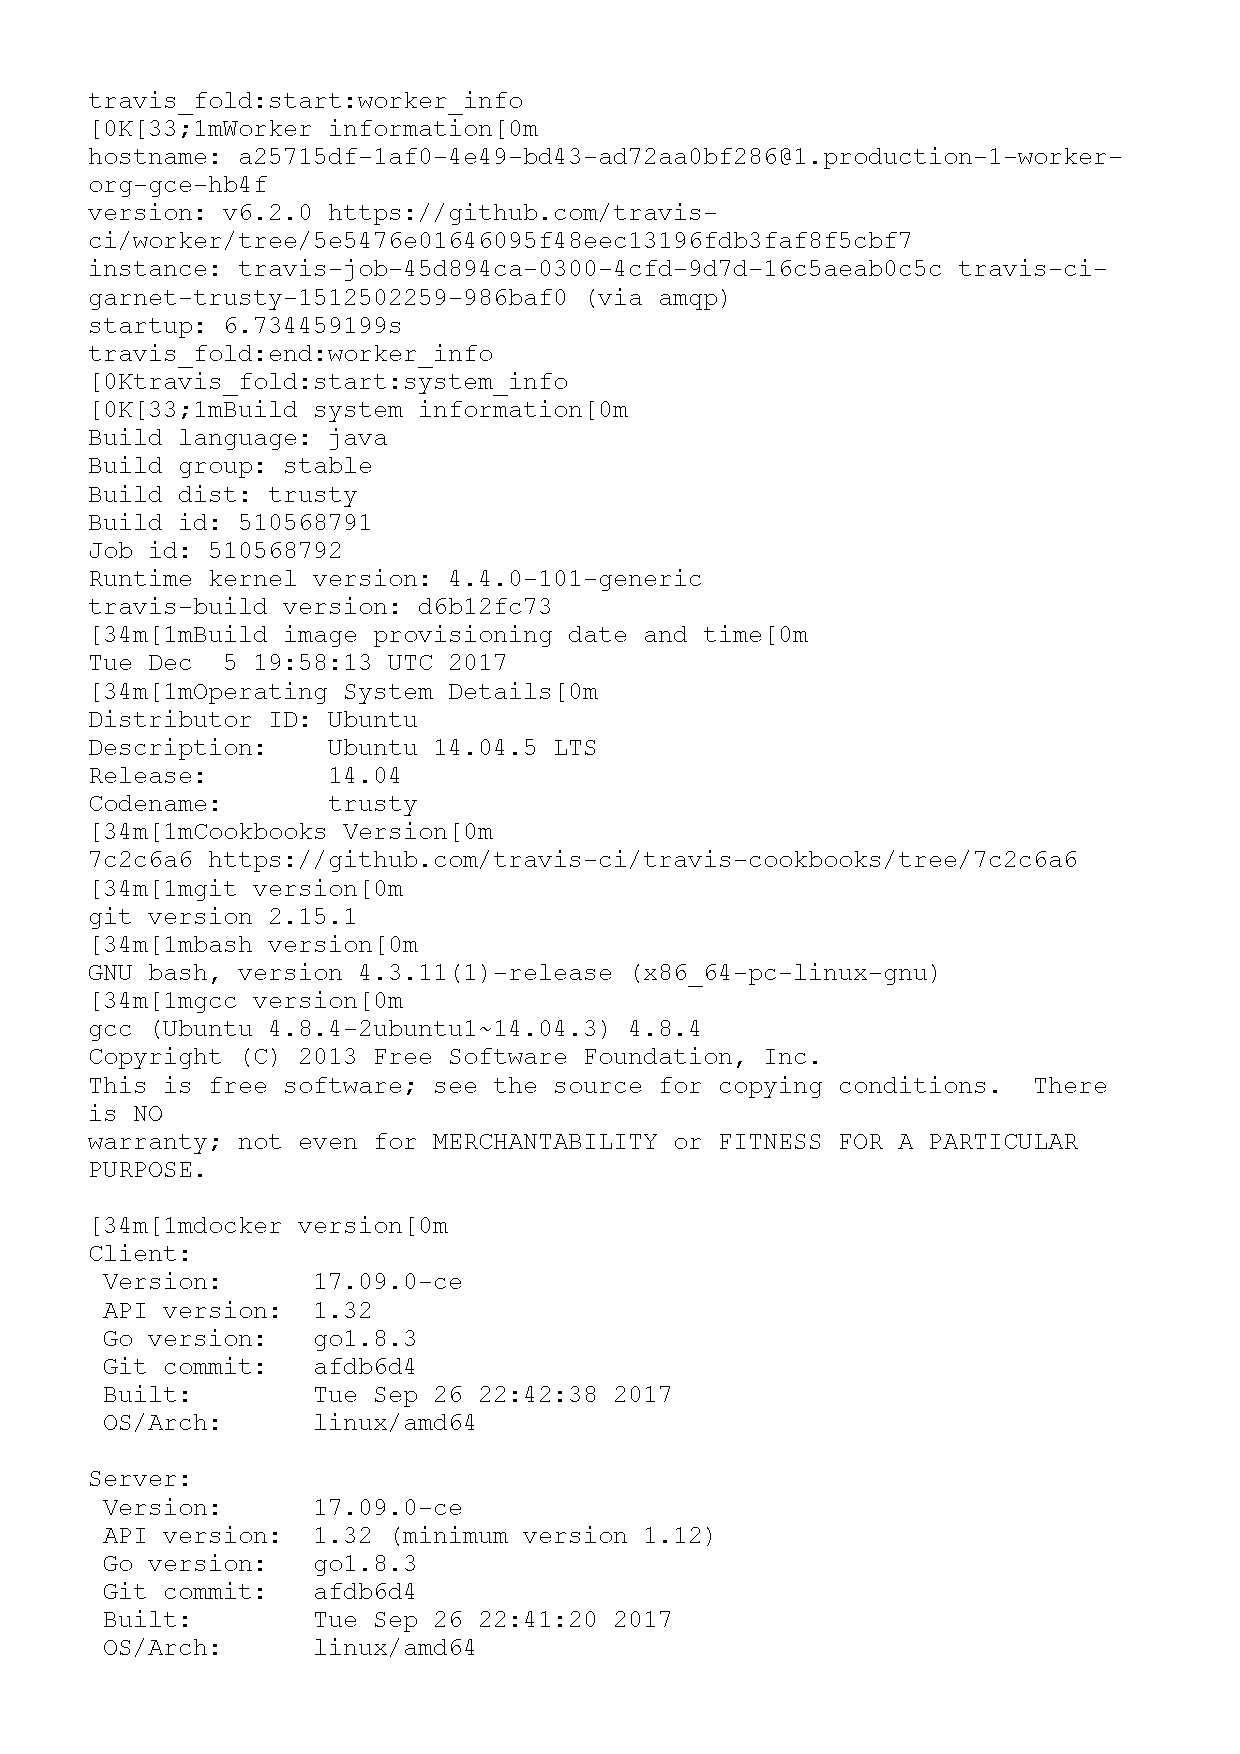
\includepdf[pages=-,scale=.9]{Build453_failed.pdf}

\subsection{Build457 passed}

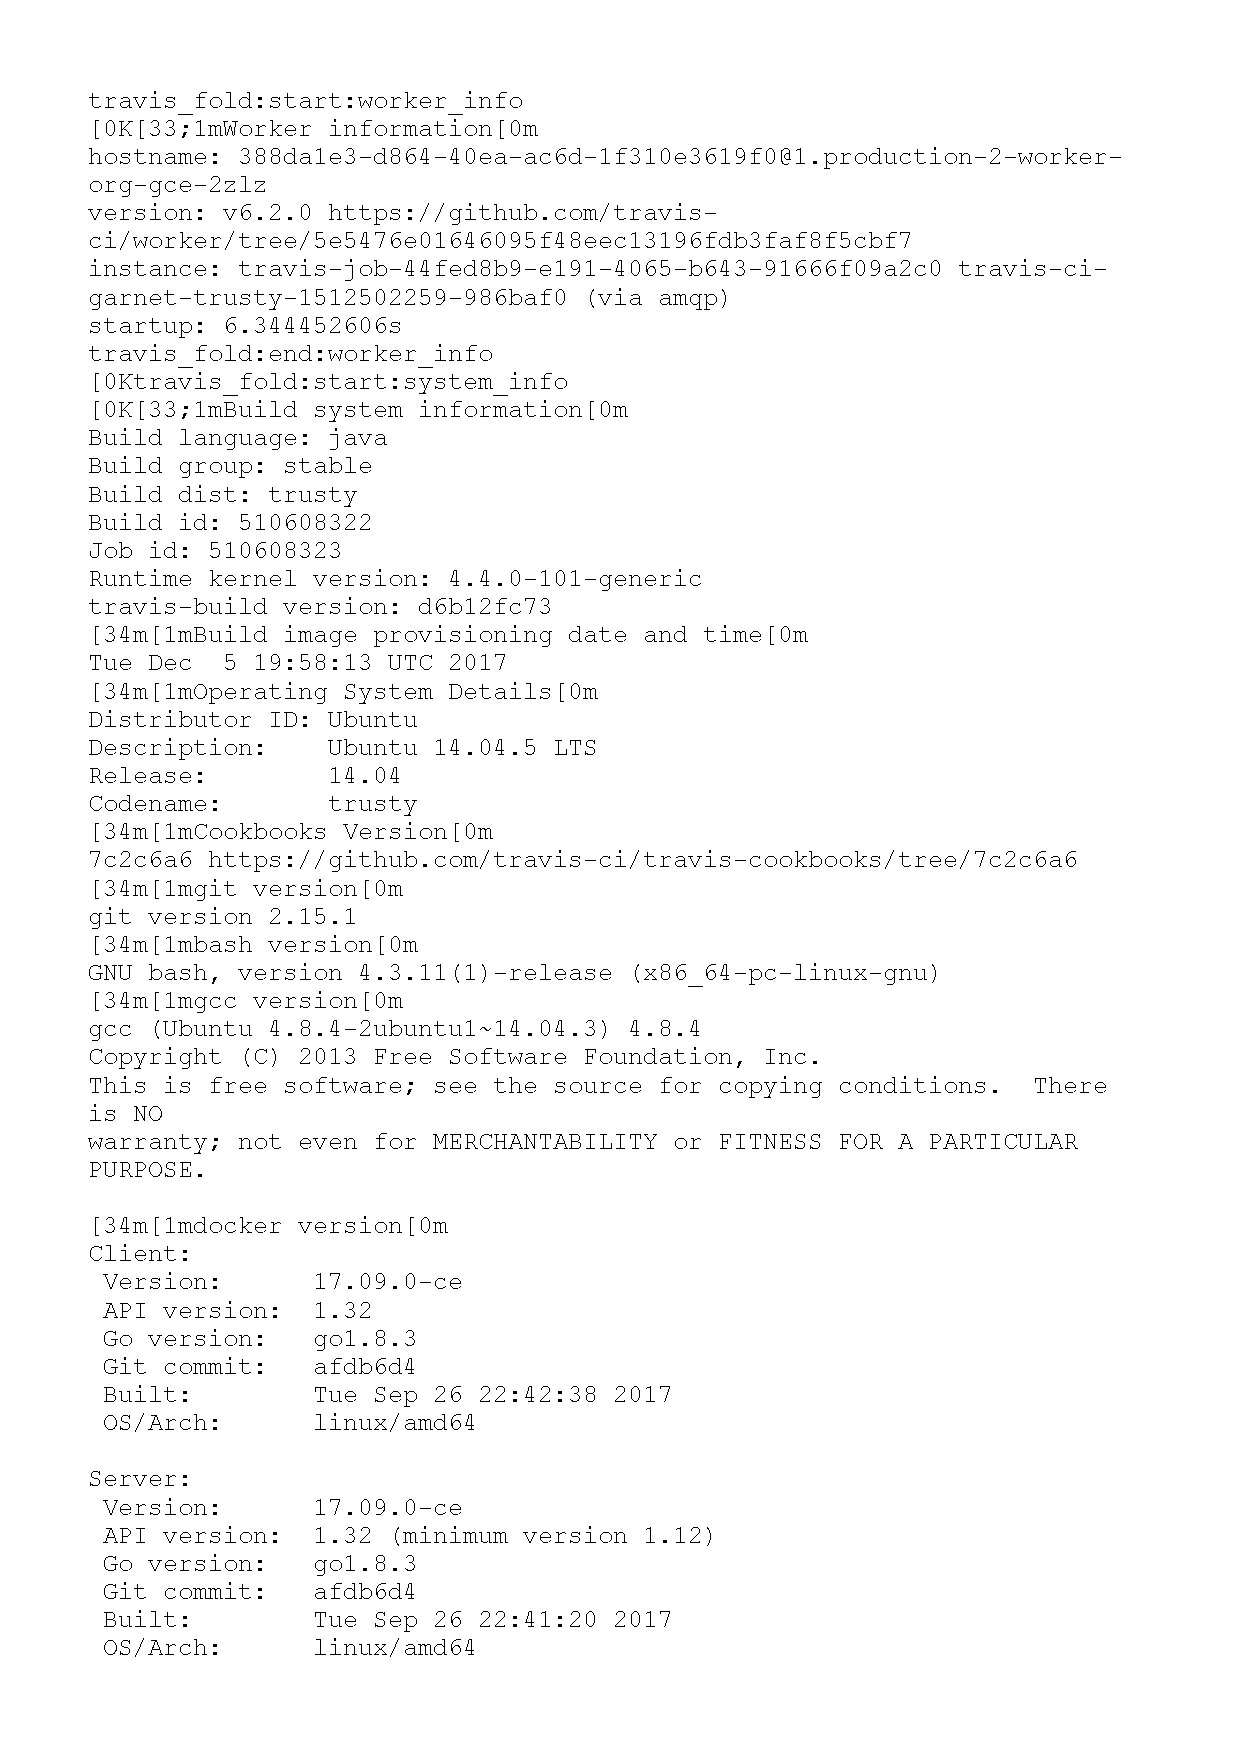
\includepdf[pages=-,scale=.9]{Build457_passed.pdf}


\end{document}
